%----------------------------------------------------------------------------------------
% PACKAGES AND OTHER DOCUMENT CONFIGURATIONS
%----------------------------------------------------------------------------------------

% !TEX encoding = UTF-8
% !TEX TS-program = pdflatex
% !TEX root = data mining.tex
% !TEX spellcheck = it-IT

\documentclass[a4paper, 11pt]{report} % Font size (can be 10pt, 11pt or 12pt) and paper size (remove a4paper for US letter paper)
\usepackage[italian]{babel}      							% Lingua italiana
\usepackage[margin=1.2in]{geometry}             % Imposta i margini del documento

\usepackage[T1]{fontenc} % Required for accented characters
\usepackage[mathletters]{ucs}    % Caratteri matematici come UTF8
\usepackage[utf8]{inputenc}      % Ancora utf8

\usepackage{eurosym}                %simbolo dell'euro
\usepackage{listings}
\usepackage[usenames,dvipsnames,svgnames,table]{xcolor}
% Imposta lo spazio nella list of listing in modo simile alla list of figures/tables
%\makeatletter
%\let\my@chapter\@chapter
%\renewcommand*{\@chapter}{%
%  \addtocontents{lol}{\protect\addvspace{10pt}}%
%  \my@chapter}
%\makeatother


\definecolor{codegreen}{rgb}{0,0.6,0}
\definecolor{codegray}{rgb}{0.5,0.5,0.5}
\definecolor{backcolor}{rgb}{0.98,0.98,0.98}

\renewcommand{\lstlistingname}{Codice}% Listing -> codice
\renewcommand{\lstlistlistingname}{Elenco dei frammenti di codice}% List of Listings -> Frammenti di codice

\lstdefinestyle{mystyle}{
    backgroundcolor=\color{backcolor},   
    commentstyle=\color{Peach}\ttfamily,
    keywordstyle=\color{RoyalBlue},
    numberstyle=\tiny\color{codegray},
    stringstyle=\color{SeaGreen}\ttfamily,
    basicstyle=\footnotesize\ttfamily,
    breakatwhitespace=false,         
    breaklines=true,                 
    captionpos=b,                    
    keepspaces=true,                 
    numbers=left,                    
    numbersep=5pt,                  
    showspaces=false,                
    showstringspaces=false,
    showtabs=false,                  
    tabsize=2,
    frame=trbl, % draw a frame at the top, right, left and bottom of the listing
	frameround=ftff, % angolo in basso a destro curvo
	framesep=4pt, % quarter circle size of the round corners,
	inputencoding=utf8,
    extendedchars=true,
    literate={á}{{\'a}}1 {à}{{\`a}}1 {é}{{\'e}}1 {è}{{\`e}}1 {ù}{{\`u}}1 {ò}{{\`o}}1 {ì}{{\`i}}1,
    belowskip=1em,
    aboveskip=1em,
}

 
\lstset{style=mystyle}

\lstdefinelanguage{JavaScript}
{
  % list of keywords
  morekeywords={ true, false, catch, function, break,	new, class, extends, var, require, switch, return, import, if, while, for, this, View, Text, StyleSheet},
  sensitive=false, % keywords are not case-sensitive
  morecomment=[l]{//}, % l is for line comment
  morecomment=[s]{/*}{*/}, % s is for start and end delimiter
  morestring=[b]' % defines that strings are enclosed in double quotes
}

\lstdefinelanguage{JSON}
{
  % list of keywords
  morekeywords={string, boolean, int, Array, Node, Asset, AssetDetail, Filter, FilterItem},
  sensitive=false, % keywords are not case-sensitive
  morecomment=[l]{//}, % l is for line comment
  morecomment=[s]{/*}{*/}, % s is for start and end delimiter
  morestring=[b]" % defines that strings are enclosed in double quotes
}

\lstdefinelanguage{URM}
{
	% list of keywords
	morekeywords={ S, J, T, Z, I},
	sensitive=false, % keywords are not case-sensitive
	morecomment=[l]{//}, % l is for line comment
	morecomment=[s]{/*}{*/}, % s is for start and end delimiter
	morestring=[b]' % defines that strings are enclosed in double quotes
}

\lstdefinelanguage{RDFA}{
	language=html,
	sensitive=true, 
	alsoletter={<>=-},
	ndkeywords={
		% General
		=,
		% HTML attributes
		charset=, id=, width=, height=, property=, about=, rel=, rev=, prefix=, vocab=, content=, datatype=
	},  
	morecomment=[s]{<!--}{-->},
	tag=[s]
}

%\tightlist per compatibilità con pandoc
\providecommand{\tightlist}{%
  \setlength{\itemsep}{0pt}\setlength{\parskip}{0pt}}


\usepackage[labelfont=bf]{caption}

\usepackage[protrusion=true,expansion=true]{microtype} % Better typography
\usepackage{graphicx} % Required for including pictures
\usepackage{wrapfig} % Allows in-line images


\usepackage{subfig}
\usepackage{hyperref}
\usepackage{mathpazo} % Use the Palatino font

\linespread{1.05} % Change line spacing here, Palatino benefits from a slight increase by default
\usepackage{placeins}
\usepackage{sourcecodepro}
\usepackage{hyperref}                   % collegamenti ipertestuali

\usepackage[colorinlistoftodos,prependcaption]{todonotes} %todo

\usepackage{amsmath}

\usepackage{float}
\usepackage{algorithm}
\usepackage{algpseudocode} % https://en.wikibooks.org/wiki/LaTeX/Algorithms#Typesetting_using_the_algorithmicx_package

\makeatletter
\renewcommand\@biblabel[1]{\textbf{#1.}} % Change the square brackets for each bibliography item from '[1]' to '1.'
\renewcommand{\@listI}{\itemsep=0pt} % Reduce the space between items in the itemize and enumerate environments and the bibliography


\newcommand{\cov}{\text{cov}}
\newcommand{\var}{\text{var}}

\renewcommand{\maketitle}{ % Customize the title - do not edit title and author name here, see the TITLE block below
\begin{flushright} % Right align
{\LARGE\@title} % Increase the font size of the title

\vspace{50pt} % Some vertical space between the title and author name

{\large\@author} % Author name
\\\@date % Date

\vspace{100pt} % Some vertical space between the author block and abstract
\end{flushright}
}

%% breakablealgorithm http://tex.stackexchange.com/questions/33866/algorithm-tag-and-page-break
\makeatletter
\newenvironment{breakablealgorithm}
{% \begin{breakablealgorithm}
	\begin{center}
		\refstepcounter{algorithm}% New algorithm
		\hrule height.8pt depth0pt \kern2pt% \@fs@pre for \@fs@ruled
		\renewcommand{\caption}[2][\relax]{% Make a new \caption
			{\raggedright\textbf{\ALG@name~\thealgorithm} ##2\par}%
			\ifx\relax##1\relax % #1 is \relax
			\addcontentsline{loa}{algorithm}{\protect\numberline{\thealgorithm}##2}%
			\else % #1 is not \relax
			\addcontentsline{loa}{algorithm}{\protect\numberline{\thealgorithm}##1}%
			\fi
			\kern2pt\hrule\kern2pt
		}
	}{% \end{breakablealgorithm}
	\kern2pt\hrule\relax% \@fs@post for \@fs@ruled
\end{center}
}
\makeatother

%----------------------------------------------------------------------------------------
% TITLE
%----------------------------------------------------------------------------------------

\title{\textbf{Data Mining}\\ % Title
A.A. 2015-2016} % Subtitle

\author{\textsc{Giacomo Manzoli}
\\ 1130822 % Author
\\{\textit{Università degli Studi di Padova}}} % Institution

\date{\today} % Date

%----------------------------------------------------------------------------------------

\begin{document}

\maketitle % Print the title section

%----------------------------------------------------------------------------------------
% ABSTRACT AND KEYWORDS
%----------------------------------------------------------------------------------------

%\renewcommand{\abstractname}{Summary} % Uncomment to change the name of the abstract to something else

\clearpage
\tableofcontents
%\listofalgorithms

%\hspace*{3,6mm}\textit{Keywords:} lorem , ipsum , dolor , sit amet , lectus % Keywords

\vspace{30pt} % Some vertical space between the abstract and first section

%----------------------------------------------------------------------------------------
% ESSAY BODY
%----------------------------------------------------------------------------------------
\clearpage

% !TEX encoding = UTF-8
% !TEX program = pdflatex
% !TEX root = MEMOC.tex
% !TEX spellcheck = it-IT

% 6 Ottobre 2016

\chapter{Introduzione}

Il corso è in inglese, ma il contenuto non cambia rispetto l'anno scorso. Anche il materiale fornito sarà in inglese. La mail del docente è \url{luigi@math.unipd.it}. C'è anche il professore Di Summa che farà il laboratorio.

La pagina del corso è \url{http://www.math.unipd.it/~luigi/courses/metmodoc/metmodoc.html}.

\section{Obiettivo del corso}

L'obiettivo del corso è quello di introdurre delle tecniche avanzate per la modellazione e risoluzione di problemi di ottimizzazione combinatoria.
Si tratta di problemi in cui si vuole ottimizzare un certo criterio trovando una combinazione ottima di risorse da utilizzare.

Il corso vuole fornire gli strumenti matematici e algoritmici per risolvere questo tipo di problemi, concentrandosi per lo più su problemi pratici, che verranno risolti utilizzando vari software.

Un esempio di problemi è dato da quello del telefono, ci sono delle risorse limitate per creare due possibili modelli di telefoni che vengono commercializzati a prezzi diversi. Si vuole trovare il numero di telefoni di ciascun modello da produrre per ottenere il maggior guadagno possibile in funzione delle risorse a disposizione.

\begin{figure}[htbp]
\centering
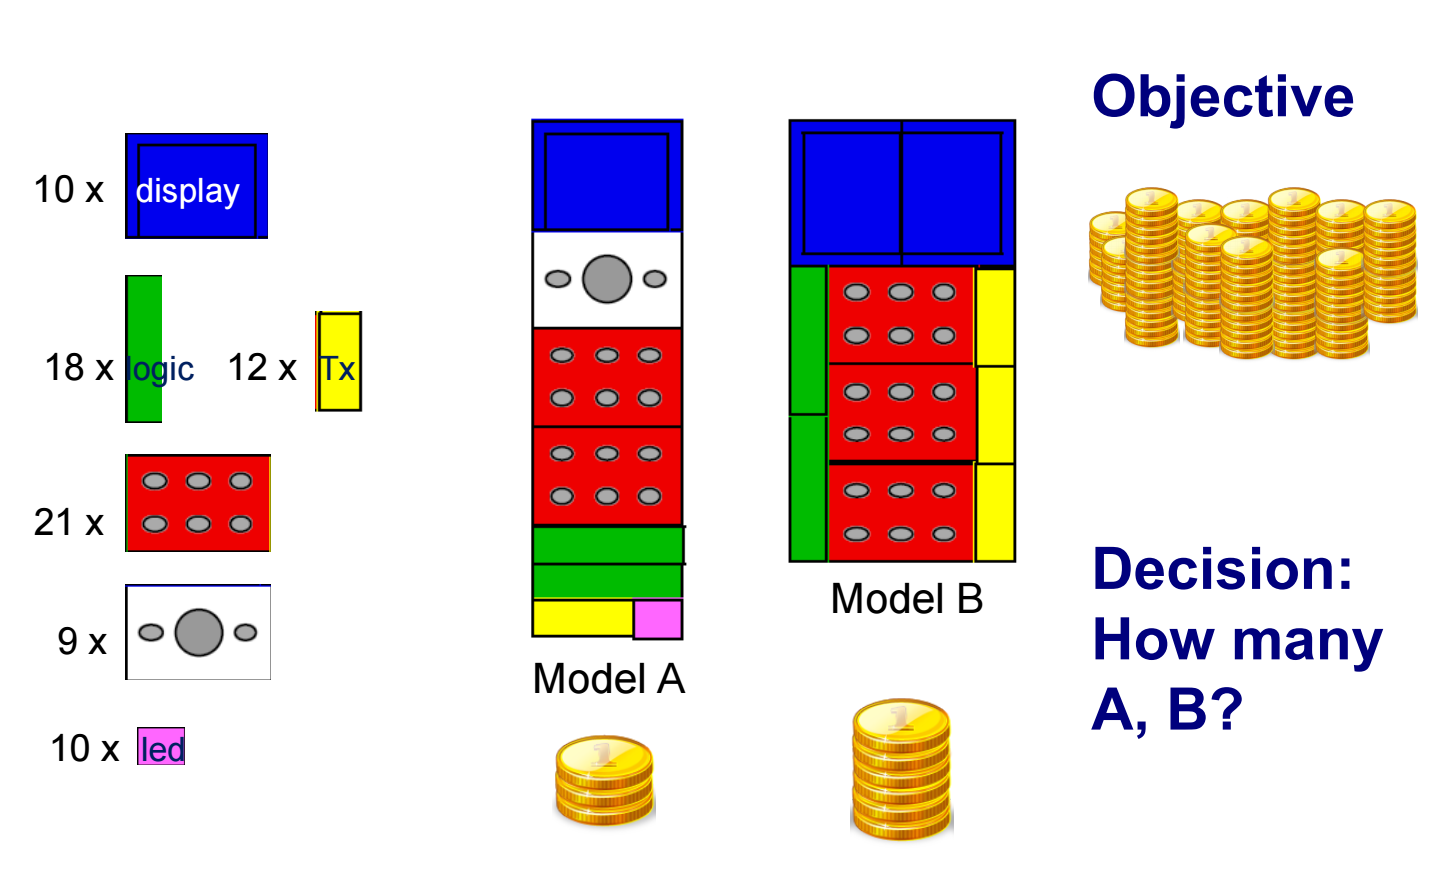
\includegraphics[width=0.7\textwidth]{images/l1-telefono.png}
\end{figure}

Per risolvere questo problema si possono usare varie strategie:

\begin{itemize}
	\item \textbf{Greedy}: scelgo di costruire il massimo numero di telefoni del modello con il prezzo più alto. Però non ho la garanzia che la soluzione trovata sia ottima.
	\item \textbf{Local search}: determino un certo numero di telefoni da produrre in modo da trovare una possibile soluzione sub-ottima per poi andare a modificare il numero di telefoni prodotti, cercando di migliorare il guadagno. Anche in questo caso non ho la garanzia che la soluzione trovata sia ottima.
	\item \textbf{Global search}: provo tutte le possibili combinazioni di telefoni che posso produrre, così facendo sono sicuro di trovare una soluzione ottima.
\end{itemize}


Un altro possibile problema è quello del contadino che possiede 12 ettari di terra dove può coltivare patate o pomodori, avendo a disposizione 70kg di semi di pomodoro, 18 tonnellate di tuberi di patate e 160 tonnellate di fertilizzante. Il contadino sa che un ettaro di campo coltivato a pomodori produce un guadagno di 3000 euro mentre uno di patate 5000. Per coltivare un ettaro a pomodori servono 7kg di semi e 10 tonnellate di fertilizzante, mentre un ettaro di patate richiede 3 tonnellate di tuberi e 20 di fertilizzante.

Questo problema è simile a quello del telefono, con la differenza che in questo caso gli ettari possono essere frazionati e quindi l'approccio combinatorio non può essere utilizzato.

L'idea è quindi quella di formulare un modello che descrive la soluzione ottima, anziché formulare un algoritmo che lo risolve.

Come prima cosa è necessario identificare le \textbf{variabili decisionali}, in questo caso $x_T$ e $x_P$ che rappresentano gli ettari coltivati. 
Poi si deve definire la \textbf{funzione obiettivo} che si vuole ottimizzare, in questo caso $\max 3000 x_T + 5000 x_P$.
Infine è necessario definire i \textbf{vincoli del problema} per modellare il consumo di risorse. In questo caso:

\begin{align*}
	x_T + x_P &\leq 12 \text{ vincolo sulla terra} \\
	7 x_T &\leq 70   \text{ vincolo sui semi di pomodoro} \\
	3 x_P &\leq 18 \text{ vincolo sui tuberi} \\
	10 x_T + 20 x_P &\leq 160 \text{ vincolo sul fertilizzante} 
\end{align*}

Con questa formulazione del problema non dico niente riguardo la soluzione del problema, ma posso utilizzare il modello creato per trovarla utilizzando dei metodi matematici dato che l'insieme di vincoli può essere visto come un sistema di disequazioni.

Un primo approccio è quello di partire da un valore di partenza della funzione obiettivo, ad esempio 27000 e provare a migliorarlo utilizzando la discesa di gradiente, fino a trovare un punto del piano che corrisponde ad un valore ottimo.
Con questo approccio posso anche dire che la soluzione trovata è ottima, perché tutte le altre soluzioni migliori richiedono un maggior numero di risorse.

\begin{figure}[htbp]
	\centering
	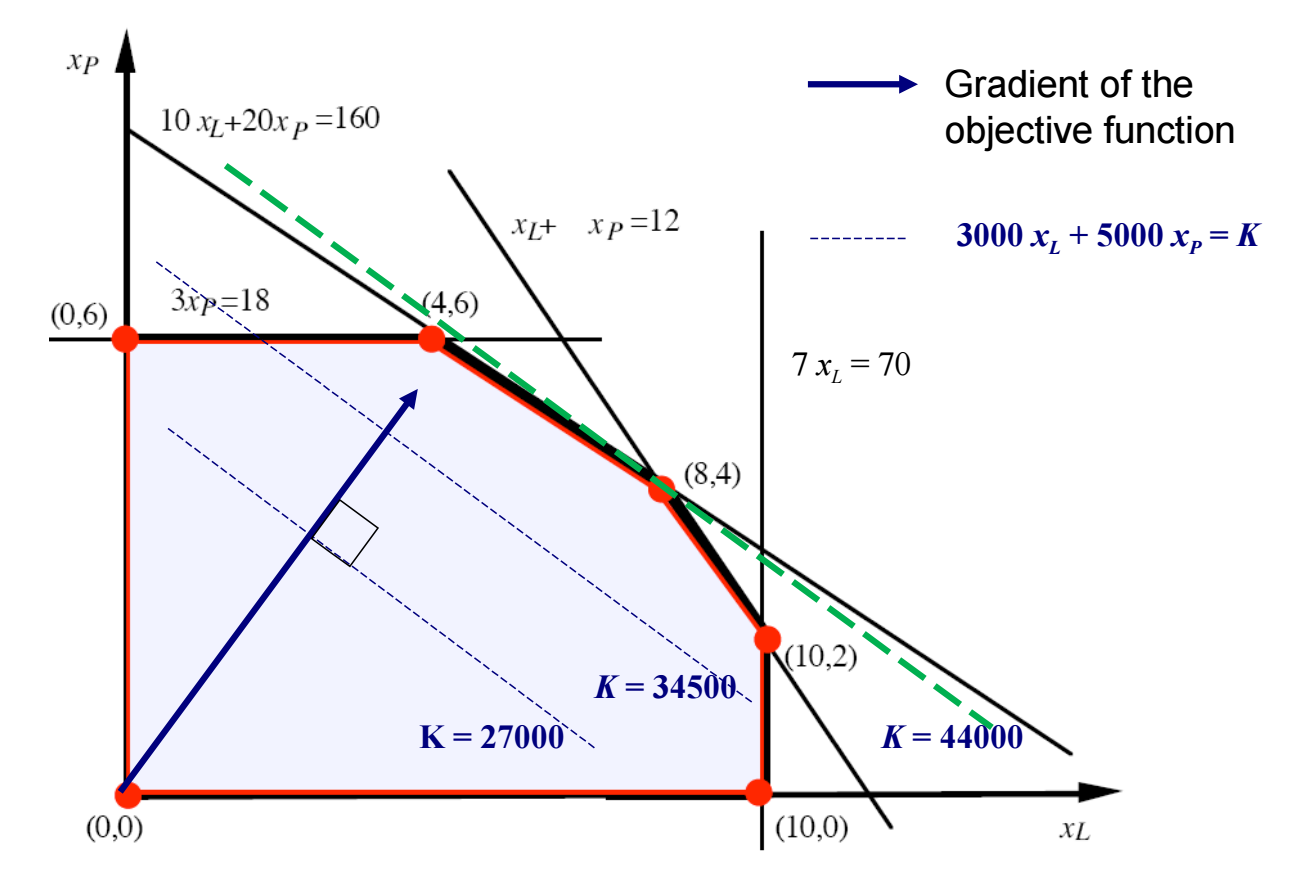
\includegraphics[width=0.5\textwidth]{images/l1-poligono.png}
\end{figure}


Tutto questo funziona perché sia i vincoli che la funzione obiettivo sono \textbf{lineari} e le variabili sono numeri reali. Questo tipo di modelli prende quindi il nome di \textbf{Linear Programming}.

Da notare che in questo caso la soluzione ottima è su un vertice intero, ma è un caso. Se le variabili utilizzate possono essere solo intere la situazione diventa più complessa perché è necessario effettuare delle approssimazioni.

\section{Approccio della ricerca operativa}

\begin{figure}[htbp]
	\centering
	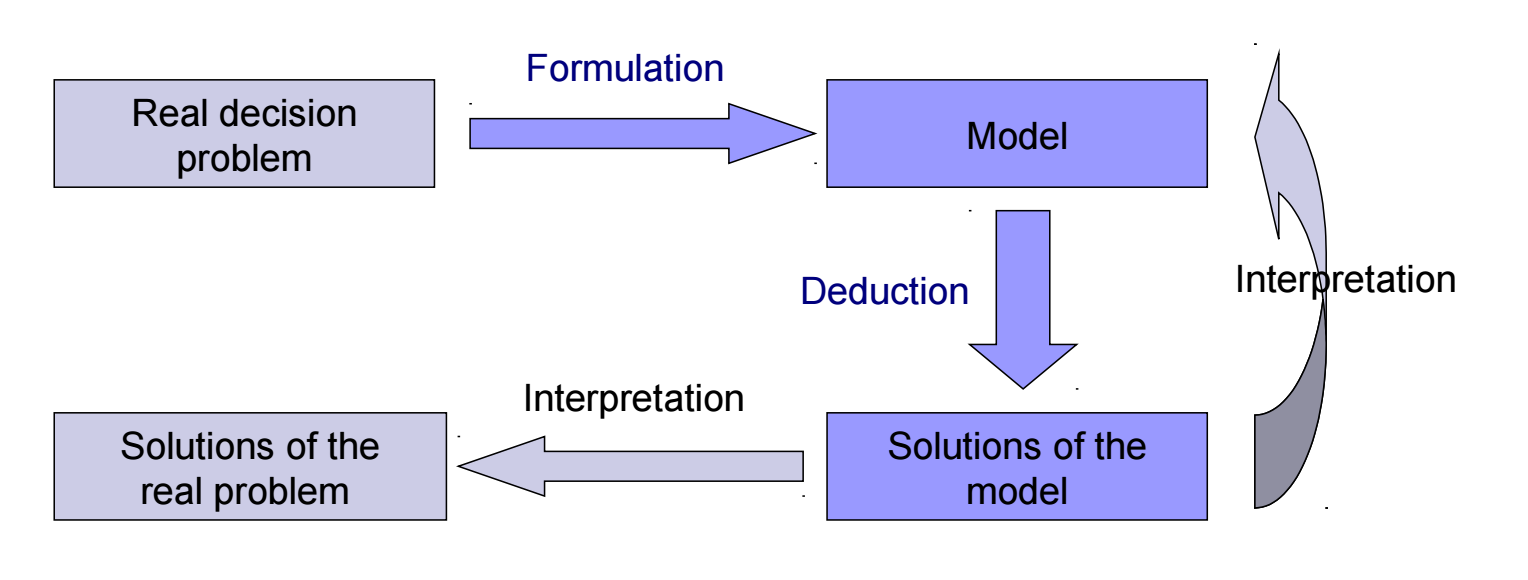
\includegraphics[width=0.7\textwidth]{images/l1-approccio.png}
\end{figure}

L'approccio precedentemente descritto è quello della ricerca operativa: si parte da un problema reale che viene formalizzato utilizzando un modello. Dal modello viene trovata una soluzione ottima per esso, la quale deve poi essere trasformata nella soluzione del problema reale.
Questo secondo passo può essere necessario perché nel modellare il problema può essere che sia stato necessario modificare alcuni vincoli, oppure utilizzare delle variabili reali anziché intere.

Si possono quindi definire due fasi: una di \textbf{formulazione} del modello e una di \textbf{deduzione} della soluzione, utilizzando alcuni algoritmi già definiti o personalizzati.

\section{Programma del corso}

\begin{enumerate}
	\item Ripasso e approfondimento delle tecniche di programmazione lineare e della dualità.
		\begin{itemize}
			\item Modelli LP, metodo del simplesso, teorema della dualità.
			\item Column generation technique per modelli LP grandi. Ovvero la creazione di modelli dinamici per evitare le limitazioni della memoria.
			\item Applicazioni: pianificazione della produzione, gestione del flusso di rete.
		\end{itemize}
	\item Metodi avanzati per la programmazione lineare intera mista (\textbf{MILP}).
		\begin{itemize}
			\item Formulazioni alternative, Branch \& Bound, Branch \& Cut.
			\item Applicazioni: Traveling Salesman Problem, localizzazione dei magazzini, set cover.
		\end{itemize}
	\item Meta euristiche per l'ottimizzazione combinatoria.
		\begin{itemize}
			\item Neighbourhood search e varianti.
			\item Algoritmi genetici.
		\end{itemize}
	\item Network optimization: modellazione dei problemi di ottimizzazione con i grafi. \textit{Potrebbe non essere affrontato.}
	\item \textbf{Laboratorio}:
		\begin{itemize}
			\item Online optimization server
			\item Optimization software and Algebraic modelling languages
			\item Optimization libraries (Cplex, Coin-OR, Scip)
		\end{itemize}
\end{enumerate}


\section{Informazioni pratiche}

Ci saranno dei laboratori nell'orario delle lezioni, verrà specificato nel sito quando ci saranno.

Non ci sono libri, vengono fornite le dispense dal professore e saranno in inglese.

Per ottenere il software che verrà utilizzato il laboratori è necessario registrarsi sul sito \url{http://www.math.unipd.it/userlist/subscribe/?idlist=277}, utilizzando la chiave \texttt{MeMoCO.16}. Per scaricare gratuitamente CPlex Optiumization Suite è necessario registrarsi alla IBM Academic Initiative.

L'esame è composto da:

\begin{itemize}
	\item Due esercitazioni di laboratorio, una sulla modellazione MILP e una sulle meta-euristiche, da consegnare qualche giorno prima dell'orale. Da fino a 10 punti.
	\item Esame orale che consiste nella discussione delle esercitazioni di laboratorio e delle domande teoriche sui contenuti del corso. Da fino a 20 punti. Forse si può fare in italiano.
	\item Progettino opzionale per ottenere un bonus da 2 a 6 punti. Il progetto riguarda la modellazione di un problema accordato con il docente e risolto utilizzando delle meta-euristiche o in modo esatto. Può essere fatto anche dopo lo scritto.
\end{itemize}



% !TEX encoding = UTF-8
% !TEX program = pdflatex
% !TEX root = AALP.tex
% !TEX spellcheck = it-IT

% 6 Ottobre 2016

\chapter{Il mini linguaggio funzionale}

\section*{Testi di riferimento}

\begin{itemize}
	\item Types and Programming Languages (B. Pierce) 
	\item Practical Foundations for Programming Languages - Capitoli 1 e 2, consigliato leggerli prima della prossima lezione
\end{itemize}

\section{Teoria dei linguaggi di programmazione}

Si vuole descrivere il comportamento dei programmi in un modo preciso e formale, definendo una sintassi e una semantica.
Definire la sintassi è abbastanza semplice, la semantica è invece più complessa perché può avere varie sfumature:

\begin{itemize}
	\item \textbf{Semantica operazionale}: descrive come evolve la computazione del programma.
	\item \textbf{Semantica denotazionale}: descrive il programma in termini matematici, come una relazione tra l'input e l'output.
	\item \textbf{Semantica assiomatica}: descrive il programma utilizzando delle proprietà che sono vere per un certo programma, per poi utilizzarle per derivarne di nuove.
\end{itemize}

\noindent Noi ci concentreremo sulla semantica operazionale che viene verificata mediante tecniche di analisi statica sfruttando: sistemi di tipi, logiche temporali e interpretazione astratta.
Una volta fissato un sistema di tipi, questa verifica del programma può anche essere automatizzata.

\section{Linguaggi funzionali}

Studiare i tipi risulta più semplice sui linguaggi funzionali che su quelli imperativi.
Inoltre, lo stile di programmazione funzionale risulta più elegante perché è concentrato sul \textit{``what to do''} anziché \textit{``how to do''}.

\begin{lstlisting}[language=Java, caption=Confronto tra Java 5 e Java 8: nel secondo caso è subito chiaro l'intento del programmatore inoltre non vengono aggiunte variabili \textit{mutable}. Tuttavia l'esempio non usa le caratteristiche funzionali di Java8]
// Java 5
boolean found = false;
for(String city : cities){
	if (city.equals("Chicago")) {
		found=true;
		break;
	}
}
System.out.println("Found?" + found);
	
// Java 8
System.out.println("Found?" + cities.contains("Chicago"));
\end{lstlisting}

\begin{lstlisting}[language = Java, caption=Confronto tra Java 5 e Java 8: l'utlilizzo delle funzioni lambda rende il codice più conciso. Inoltre non vengono usate variabili mutabili e il codice è facilmente parallelizzabile.]
// Java 5
Collection<Person> people = ...;
int maxAge = -1;
for (Person p : people) {
	if (p.getGender() == MALE && p.getAge() > maxAge){
		maxAge = p.getAge();
	}
}

// Java 8
Collection<Person> people = ...;
final int maxAge = people.stream()
										      .filter(p -> p.getGender() == MALE)
										      .mapToInt(p -> p.getAge())
										      .max();
\end{lstlisting}

\noindent Tra le caratteristiche distintive dei linguaggi funzionali c'è l'\textbf{assenza degli assegnamenti}: ci sono delle variabili ma queste rappresentano dei valori e non delle aree di memoria modificabili. Vengono quindi solamente rappresentati dei valori immutabili.

Segue quindi che non ci sono side-effects: la chiamata di una funzione può essere sostituita con il suo risultato (\textbf{referential transparency}). Questo non è più valido se ad esempio la funzione stampa qualcosa a video e poi ritorna un risultato, pertanto se una funzione è pura, questa non può neanche produrre delle stampe a video.

Sembra una limitazione, ma in realtà così facendo si hanno vari vantaggi:
\begin{itemize}
	\item Il codice diventa più affidabile e più riusabile.
	\item Due funzioni che lavorano su dati diversi come \texttt{f(x)} e \texttt{g(y)} possono essere eseguite in parallelo senza problemi.
	\item Tutto ciò che entra ed esce dalla funzione può essere sottoposto a type check e quindi al compilatore basta solo il prototipo. Inoltre, se c'è un errore logico nella definizione della funzione è facile che questo si rifletta anche in un errore di tipo.
\end{itemize}

\noindent Un'altra caratteristica chiave è che le funzioni sono oggetti \textbf{first class}, ovvero sono a tutti gli effetti degli oggetti che possono essere passati come parametro ad altre funzioni. 
Le funzioni che prendono in input altre funzioni vengono chiamate funzioni \textbf{higher order}.
Ciò permette di scomporre un problema in sotto-problemi, utilizzare delle funzioni semplici per risolvere i sotto-problemi, per poi combinare le funzioni utilizzando delle funzioni higher-order.

\section{Sintassi del nostro linguaggi $\mathcal{L}$}

\begin{align*}
	x \in Var & &\\
	n \in Num & &\\
	Termini \: M, N &::= x &\text{ variabili} \\
								&|\: n \:|\: \text{true} \:|\: \text{false} &\text{ costanti intere e booleane} \\
								&|\: M + M \:|\: M - M &\text{ operazioni intere} \\
								&|\: \text{if} \: M \: \text{then} \: M \: \text{else} \: M &\text{ condizionale} \\
								&|\: \text{fn } x.M &\text{ dichiarazione di una funzione} \\
								&|\: M \: M &\text{ applicazione di una funzione}
\end{align*}

\noindent Un programma è quindi un termine chiuso \textit{M}, ovvero che non ha variabili libere e l'esecuzione del programma equivale a trovare il valore del termine \textit{M}.

Alcuni esempi di programmi:

\begin{align*}
3 + 2 &\\
\text{fn} \:  x.x &\:\text{// funzione identità} \\
\text{fn} \: x.3 &\: \text{// funzione costante 3} \\
\text{fn} \: x.x+1 &\: \text{// funzione successore} \\
\text{fn} \: x.x+1 \: 3 &\: \text{// funzione successore applicata al numero 3} \\
\text{fn} \: x.\text{fn} \: y . x+y &\: \text{// funzione somma con due argomenti (currificata)} \\
\text{fn} \: x. (\text{fn} \: y . x+y   + 2) &\: \text{// funzione che ritorna la funzione $2+x$} \\
\underbrace{\text{fn} \: x.\text{fn}\ y.(x\: y)}_{M} &\: \text{// funzione che applica un'altra funzione} \\
(M \: \text{fn} \: z.z) \: 5 &\: \text{// applicazione della funzione identità al numero 5} \\
\text{if} \: 2 \: \text{then} \: \text{fn}\: x.x+x \: \text{else} \: 0 &\: \text{// utilizzo del condizionale, è sinteticamente corretto ma non a livello di tipi}
\end{align*}

\noindent Il comportamento dei programmi dipende poi dalla semantica che viene attribuita alle istruzioni.

\subsection{Variabili libere}

C'è poi il concetto di variabile \textbf{libera} o \textbf{legata}.
La variabile $x$ nel termine $\text{fn } x.x$ è legata, perché viene dichiarata dal termine, infatti $\text{fn}$ è un \textit{binder}.

Nel termine $x+y$ le due variabili sono libere, perché non si riesce ad attribuirgli un valore. Per funzionare un programma non deve avere variabili libere.
Mentre nel termine $\text{fn }y. x\: y$ la variabile $x$ è libera mentre la $y$ è legata. Si ottiene così una \textbf{clojure}, ovvero una funzione che per essere calcolata deve ricevere dei valori per le variabili libere.

Ci sono poi le funzioni \textbf{alpha-equivalenti}, ovvero funzioni che calcolano la stessa cosa, ma che utilizzano variabili legate con nomi diversi. Es: $\text{fn }y.y+1$ e $\text{fn }x.x+1$.

Più formalmente si possono definire le variabili libere in modo induttivo.
Dato un termine $M$, le variabili libere di $M$ vengono indicate con $fv(M)$ e sono definite induttivamente come:

\begin{align*}
	fv(x) &= \{ x \} \\
	fv(n) =fv(\text{true}) = fv(\text{false}) &= \emptyset \\
	fv(M + N) = fv(M-N) &= fv(M) \cup fv(N) \\
	fv(\text{if } M_1 \text{ then } M_2 \text{ else }M_3) &= fv(M_1) \cup fv(M_2) \cup fv(M_3) \\
	fv(\text{fn }x.M) &= fv(M) \setminus \{x\} \\
	fv(M \: N) &= fv(M) \cup fv(N)
\end{align*}

\noindent Un termine senza variabili libere viene detto \textbf{chiuso} e i programmi sono definiti da dei termini chiusi.

\subsection{Sostituzione}

Definiamo ora l’operazione di sostituzione di una variabile con un termine, necessaria per la definizione della semantica del linguaggio. 
Indichiamo con $M \{x := N\}$ il termine $M$ in cui la variabile $x$ è stata sostituita con il termine $N$.
Nel seguito useremo una notazione compatta in cui \textit{c} varia nell’insieme delle costanti intere e booleane, mentre $op(M_i)_{i\in I}$ varia nell’insieme delle operazioni aritmetiche e booleane.

\begin{align*}
	x \{x := N\} &= N \\
	y \{x := N\} &= y \\
	c \{x := N\} &= c \\
	op(M_i)_{i \in I}\{x := N\}  &= op(M_i\{x := N\} )_{i \in I} \\
	(M_1 + M_2) \{ x:= N \} &= M_1\{x := N\} + M_2 \{x := N\} \\
	(\text{fn} \: x.M)\{x := N\} &= \text{fn }x.M \\
	(\text{fn} \: y.M)\{x := N\}  &= \text{fn }y.M\{x := N\} \text{ if } y \notin fv(N) \\
	(M_1 \: M_2) \{x := N\}  &= (M_1\{x := N\} \: M_2 \{x := N\} )
\end{align*}

\noindent Quando applico una sostituzione $M\{x := N\}$ devo stare atteno a sostituire solamente le occorrenze libere di $x$ ed è inoltre importante che i termini che vado ad aggiungere non vengano catturati da un altro binder.
Per evitare questo problema è necessario rinominare le variabili problematiche per alpha conversione.

Ad esempio $(\text{fn }x.x)\{x := 3\}$ \textbf{non} è $\text{fn }x.3 $ ma $\text{fn }x.x$ e allo stesso modo $(\text{fn }y.x+y)\{x := y\}$ \textbf{non} è $\text{fn }y.y+y$ ma $(\text{fn }x.x+z)\{x := y\} = \text{fn }z.y+z$.






% !TEX encoding = UTF-8
% !TEX program = pdflatex
% !TEX root = InformationRetrieval.tex
% !TEX spellcheck = it-IT

% 6 Ottobre 2016

%\chapter{Rappresentazione dei documenti}
%\section{Analisi automatica del testo}

Tutto è iniziato quando George K. \textbf{Zipf}, uno studioso americano di linguistica ha formulato delle leggi empiriche che mettono in relazione la \textbf{frequenza di una parola} con la sua \textbf{forma} e \textbf{significato}. 
Solo in un secondo momento queste leggi sono state applicate all'indicizzazione dei documenti.

L'osservazione di partenza è stata quella che ci sono poche parole che sono veramente molto frequenti, come gli articoli, e che sono poco significative rispetto il contenuto informativo del documento. Ci sono poi tante parole poco frequenti, alcune delle quali sono fortemente correlate al contenuto informativo del documento. Il gioco è quindi quello di sfruttare al meglio tali parole.

Questo andamento può essere rappresentato graficamente, prima andando a contare le frequenze delle singole parole, per poi andare ad ordinarle da quella più frequente a quella meno frequente. La distribuzione così ottenuta è intera, ma può essere approssimata da un'iperbole.

Tipicamente in inglese:
\begin{itemize}
	\item Le due parole più frequenti sono \textit{the} e \textit{of}, mediamente sono il 10\% delle parole del documento.
	\item Le 6 parole più frequenti corrispondo a circa il 20\% delle occorrenze e le 50 parole più frequenti corrispondo a circa il 40\% dei testi. Questo deriva dal fatto che la lingua deve essere ridondante in modo che sia facile da capire.
	\item Considerando un'insieme di documenti molto ampio, circa la metà delle singole parole di quel campione compare una sola volta. Queste sono parole più significative dal punto di vista dell'informazione. Tuttavia è necessario tenere conto che in questo insieme di parole possono comparire anche gli errori di battitura.
\end{itemize}

\subsection{Legge di Zipf}

La legge di Zipf afferma che dato un campione di testi e calcolata la frequenza $f$ delle parole, una volta che si sono messe le parole in ordine decrescente di frequenza, cioè si sono ordinate le parole in base al ragno \textit{r}, la distribuzione che si ottiene ha un andamento assimilabile ad una iperbole e si ha che

$$
r \times f = k
$$

ovvero la distribuzione è data da $ f = \cfrac{k}{r}$.

Se anziché ragionare in termini di frequenza assoluta si passa a considerare quella relativa, ovvero la probabilità osservata di occorrenza della parola, la legge di Zipf può essere riscritta come 

$$
r \times P_r = c
$$

Dove $P_r$ è la probabilità di occorrenza della parola che occupa il rango $r$-esimo e $c$ è una costante ($c = 0.1$ per l'inglese).

Si ha che per la lingua inglese $c \approx 0,1$ e l'iperbole che si ottiene è riportata in figura \ref{fig:zipf}

\begin{figure}[htbp]
\centering
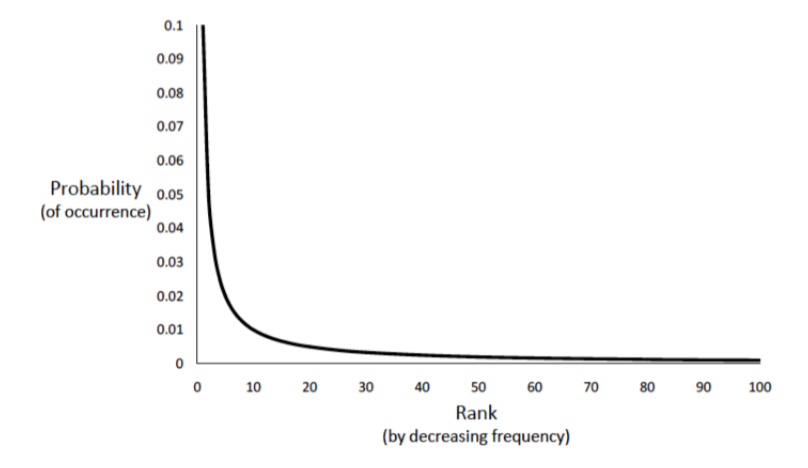
\includegraphics[width=0.55\linewidth]{images/l3-zipf}
\caption{Rango rispetto la probabilità di occorrenza assumendo valida la legge di Zipf con $c = 0.1$}\label{fig:zipf}
\end{figure}

\subsection{Indicazioni di H.P. Luhn}

L'idea per l'indicizzazione è quindi quella di definire due soglie di \textit{cut-off} per evitare di prendere in considerazione le parole troppo frequenti, perché poco significative, e quelle troppo poco, per limitare l'effetto degli errori di battitura.

Ogni parola ha un certo \textbf{resolving power}, ovvero una certa capacità di discriminare il contenuto del documento da quello degli altri e di caratterizzare il contenuto della collezione.

\begin{figure}[htbp]
	\centering
	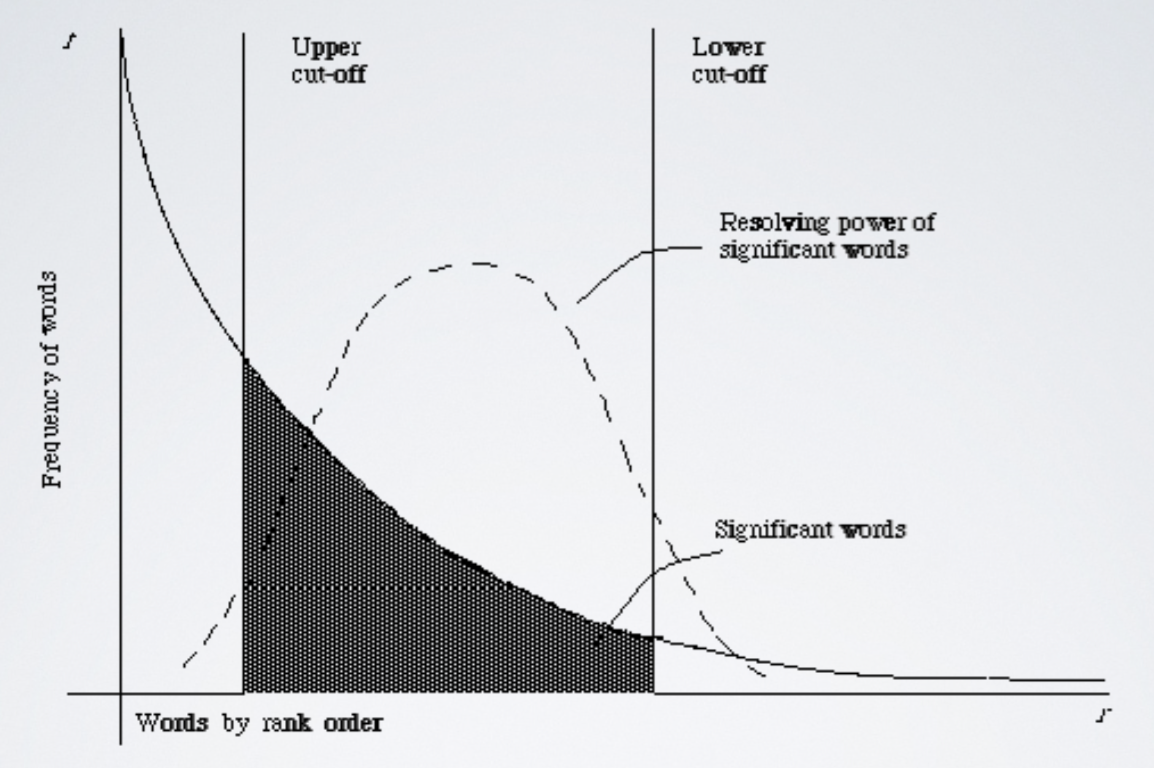
\includegraphics[width=0.55\linewidth]{images/l3-cutoff}
	\caption{Plot della curva $r \times f$ che evidenzia la posizione delle parole significative.}
\end{figure}

Questo vale per le collezioni generiche dei documenti, mentre se si parla di un argomento specifico si può dare maggiore peso a determinate parole. Ad esempio può capitare che se viene preso in esame un manuale di MySQL è ovvio che le parole ``MySQL'' e  ``table'' compariranno tante volte anche se non sono articoli.

C'è anche un altro discorso relativo alla forma plurale delle parole, che in conteggio di frequenza viene considerata come una parola diversa, quando in realtà può essere che abbia lo stesso valore informativo della forma singolare. In alcuni casi è quindi opportuno sommare le occorrenze della forma plurale e di quella singolare.

Si ha quindi che i passi per applicare le indicazioni di Luhn sono:

\begin{itemize}
	\item Si calcoli la frequenza di ogni descrittore in ogni documento della collezione di riferimento. C'è inoltre da scegliere come trattare le parti di contorno dei documenti come l'indice, la premessa, ecc. tali parti tipicamente non vengono considerate.
	\item Si calcoli la frequenza totale di ogni descrittore.
	\item Si ordino i descrittori per frequenza decrescente.
	\item Si scelga una soglia di \textit{upper cut-off} e si rimuovano dalla lista i descrittori con frequenza superiore alla soglia. In questo modo si rimuovono gli articoli, le preposizioni, ecc.
	\item Si scelga un'altra soglia di \textit{lower cut-off} e si rimuovano dalla lista i descrittori con frequenza inferiore al valore di soglia. In questo modo si rimuovono i descrittori ``rumore''  o che non apportano alcun contribuito alla descrizione del contenuto.
\end{itemize}

\noindent Entrambe le soglie possono essere calcolate in modo euristico.

Le parole che vengo eliminate dalle soglie di cut-off vengono nominate \textbf{stop word} e sono raccolte nella lista che prende il nome di \textbf{stop list}.


\textbf{{\color{Red} Possibile esercizio:}} Domande relative alle osservazioni proposte da Zipf e Luhn.

\section{Indicizzazione}

L'indicizzazione ha l'obiettivo di rappresentare il contenuto informativo di un documento e nel tempo questo processo ha preso una struttura a fasi.
Il documento viene rappresentato da dei descrittori che vengono utilizzati per la costruzione degli indici utili al reperimento dell'informazione.

Quindi l'indicizzazione fornisce automaticamente una rappresentazione più compatta e direttamente utilizzabile del contenuto informativo del documento. Gli indici sono utilizzati come surrogati del contenuto del documento durante la fase di reperimento.

L'indicizzazione può essere svolta:
\begin{itemize}
	\item manualmente
	\item in modo automatico
	\item in modo semi-automatico, quando è necessario intervenire all'interno del processo per prendere delle decisioni che non possono essere prese in modo automatico.
\end{itemize}

\noindent Tutti questi metodi funzionano estraendo direttamente dal documento le informazioni. Tuttavia possono essere estesi in modo che vengano presi in considerazione anche dei dizionari o delle meta-informazioni.

\begin{figure}[htbp]
	\centering
	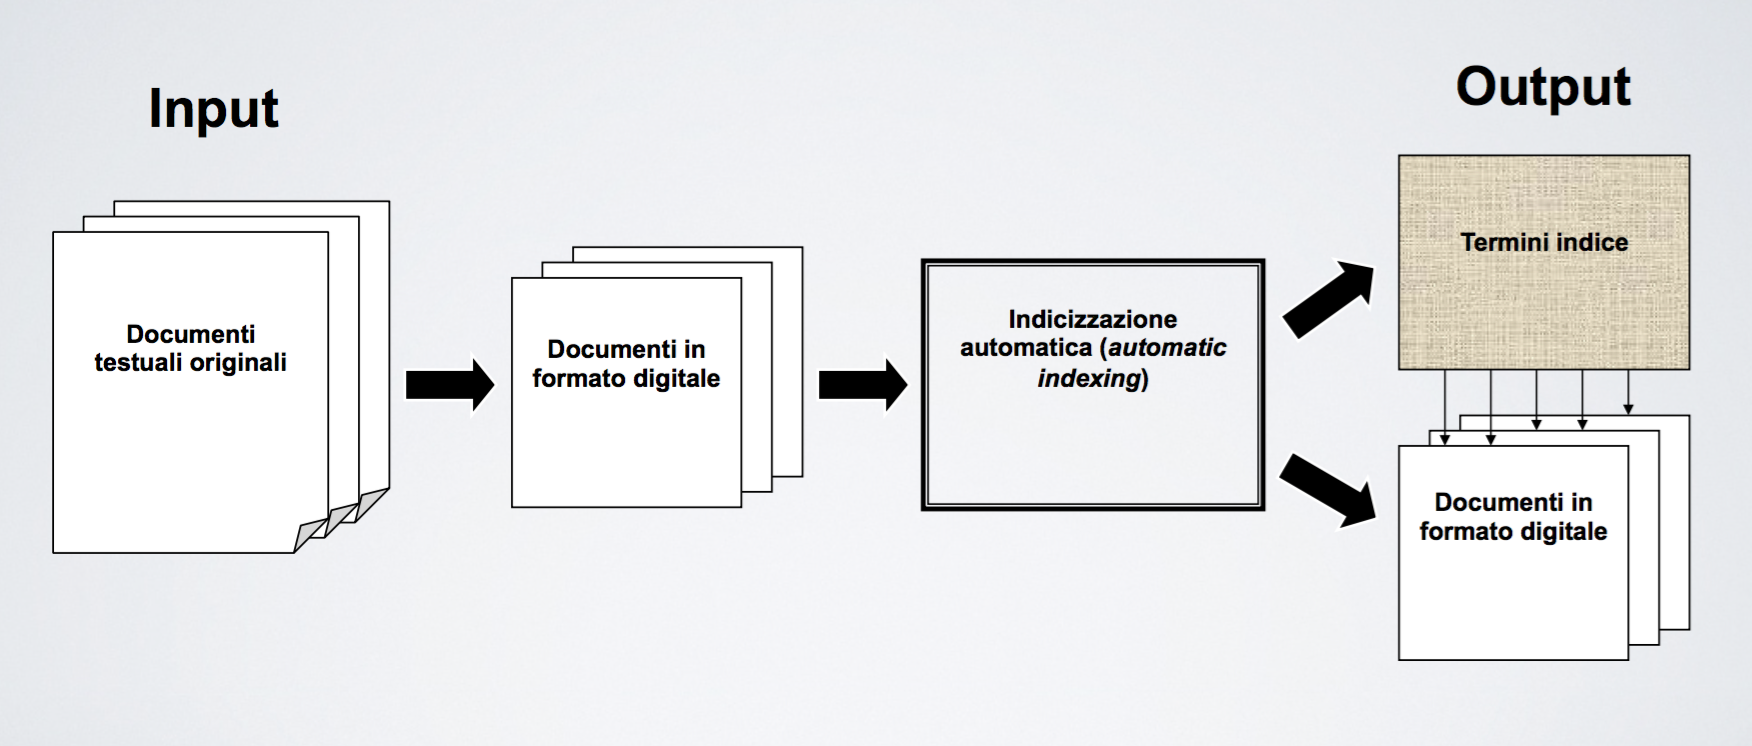
\includegraphics[width=0.7\linewidth]{images/l3-indicizzazione}
	\caption{Schema generale dell'indicizzazione}
\end{figure}

\subsection{Indicizzazione automatica dei testi}

L'indicizzazione automatica di un documento testuale è un processo che esamina automaticamente gli oggetti informativi (parole, frasi, didascalie, figure, ecc.) che compongono il documento e produce una lista di termini indice presenti nell'intera collezione dei documenti.

L'estrazione dei termini indice viene fatta da appositi algoritmi e, una volta estratti, questi vengono collegati ai diversi documenti che li contengono.
Così facendo durante il reperimento sarà sufficiente fare riferimento ai termini indice e non all'intera collezione.

\subsection{Attuazione dell'indicizzazione automatica}

L'indicizzazione automatica dei documenti testuali viene eseguita in più fasi, che devono essere attuate in sequenza:

\begin{enumerate}
	\item Analisi lessicale e selezione delle parole.
	\item Eventuale rimozione delle stop word.
	\item Riduzione delle parole originali alle rispettive radici (\textit{STEM}). Ad esempio le forme plurali vengono ridotte a quelle singolari.
	\item Composizione dei termini. Come ad esempio ``information retrieval''. Ovvero le parole vengono combinate tra loro quando si trovano ad una determinata distanza.
	\item Creazione dell'indice.
	\item Eventuale pesatura degli elementi dell'indice. 
\end{enumerate}

Alla fine di queste fasi l'indice sarà composto da parole, termini e frasi che noi riteniamo significative, assieme alle informazioni del peso che gli diamo e alla loro frequenza all'interno dei documenti.









% !TEX encoding = UTF-8
% !TEX TS-program = pdflatex
% !TEX root = ../apprendimento_automatico.tex
% !TEX spellcheck = it-IT
\section{Lezione 5 - VC-Dimension e VC-Confidence}\label{lezione-5-vc-dimension-e-vc-confidence}

\subsection{Esempi di spazi delle ipotesi}\label{esempi-di-spazi-delle-ipotesi}

Seguono alcuni esempi di spazi per le ipotesi nei problemi di
apprendimento supervisionato, cioè quei problemi in cui si vuole
stabilire se un elemento \emph{x} appartiene o meno ad una classe.

\subsubsection{Iperpiani in R2}\label{iperpiani-in-r2}

\textbf{Iperpiano}: dato uno spazio a \emph{n}-dimensioni, un iperpiano
per quello spazio è un sottospazio di dimensione \emph{n-1}. Ad esempio gli
iperpiani in $R^2$ sono tutte le rette del piano.

Lavorando in $R^2$ lo spazio delle istanze è definito come:

$$
X = \{x | x \in R^2\}.
$$

Mentre lo spazio delle ipotesi è dato dalle dicotomie indotte da iperpiani in $R^2$, cioè da tutte le possibili divisioni del piano.

$$
H = \{f_{(w,b)}(x) | f_{(w,b)}(x) = sign(w \times x + b), w \in R^2, b \in R\}
$$

Così facendo vengono prese in considerazione tutte le rette che dividono
$R^2$ in due parti in modo che da una parte l'ipotesi valga 1 e dall'altra
-1.

\subsubsection{Dischi in $R^2$}\label{dischi-in-r2}

Sempre in $R^2$ è possibile considerare come spazio delle ipotesi tutte le
dicotomie indotte da dischi in $R^2$ e centrati nell'origine.

$$
H = \{f_b(x) | f_b(x) = sign(||x||^2 - b), w \in R^2, b \in R\}
$$

Il che vuol dire che all'interno del disco le ipotesi valgono -1 mentre
al di fuori valgono 1.

\subsubsection{\texorpdfstring{Congiunzione di \emph{m} letterali positivi}{Congiunzione di m letterali positivi}}\label{congiunzione-di-m-letterali-positivi}

Lo spazio delle istanze questa volta è dato da tutte le stringhe di \emph{m} bits

$$
X = \{s | s \in \{0,1\}^m\}
$$

Lo spazio delle ipotesi è dato da tutte le sentenze logiche che
riguardano i letterali positivi $l_1$,$l_2$,\ldots{},$l_m$ ($l_i$ è vero se
l'\emph{i}-esimo bit è 1) e che contengono solo l'operatore $\wedge$.

$$
H = \{ f_{(i_1,\ldots,i_j}(s) | f_{(i_1,\ldots,i_j}(s) \text{ equivale a } l_{i_1} \wedge l_{i_2} \wedge \ldots \wedge l_{i_j}, \{i_1\ldots{}i_j\} \text{ sottoinsieme di }  \{1..m\}\}
$$

\subsection{Misurare la complessità dello spazio delle ipotesi}\label{misurare-la-complessituxe0-dello-spazio-delle-ipotesi}

Considerato un determinato spazio delle ipotesi \emph{H}, questo
contiene sempre:

\begin{itemize}
\item
  L'\textbf{ipotesi più specifica}: ipotesi più stretta e consistente con
  i dati, nell'esempio del disco è il disco più stretto in grado di
  contenere tutti i punti negativi.
\item
  L'\textbf{ipotesi più generale}: quella più grande e consistente con i
  dati, sempre nell'esempio del disco, è quello più grande
  possibile che non contiene punti positivi.
\end{itemize}

\textbf{Shattering}: (frammentazione), dato \emph{S} sottoinsieme dello
spazio delle istanze, si dice che \emph{S} è frammentato dallo spazio
delle ipotesi \emph{H} se:

$$ 
\forall S' \in S, \exists h \in H, \text{ tale che } \forall x \in S, h(x) = 1 \text{ se e solo se } x \in S'.
$$

Cioè \emph{H} realizza tutte le possibili dicotomie di \emph{S}.

\emph{H} frammenta un certo insieme \emph{S} se è possibile trovare un
iperpiano \emph{h} che raccoglie tutti i punti dell'insieme \emph{S}. Ovvero per
tutte le dicotomie di \emph{S} esiste un iperpiano che riesce a
realizzarle.

\subsubsection{VC (Vapnik-Chervonenkis) Dimension}\label{vc-vapnik-chervonenkis-dimension}

La VC-Dimension è la dimensione di uno spazio delle ipotesi \emph{H}
definito su uno spazio delle istanze \emph{X} ed è data dalla
cardinalità del sottoinsieme più grande frammentato da \emph{H}.

$$
VC(H) =
\begin{cases}
max_{S \subseteq X} |S|&\text{ tale che \emph{H} frammenta } S  \\
 \infty& \text{ se S non è limitato}
\end{cases}
$$


Ad esempio se nello spazio delle ipotesi dato dagli iperpiani su $R^2$ ho 2 punti, lo spazio delle istanze viene frammentato da
\emph{H}, perché posso sempre trovare una retta che riesce a realizzare
tutte le possibili dicotomie di due punti su un piano.
Se nello spazio delle istanze ho 3 punti, riesco comunque a realizzare
tutte le dicotomie.
Se nello spazio delle istanze ho 4 punti qualsiasi non si riesce a
trovare un iperpiano che realizza la dicotomia, quindi \emph{VC(H) =
3}.

Segue che, prendendo uno spazio delle ipotesi di cardinalità finita si
ha che:

$$
VC(H) \leq log_2(|H|)
$$

Questo perché per ogni \emph{S} frammentato da \emph{H}, abbiamo
$|H| \geq 2^{|S|}$,
cioè per ogni dicotomia in \emph{S} esiste un ipotesi in \emph{H} che la
realizza, ovvero devono essere disponibili in \emph{H} tante ipotesi
quanti sono le dicotomie in \emph{H}.

Scegliendo un \emph{S} tale che $|S| = VC(H)$, si
ottiene $|H| \geq 2^{|S|}$, prendendo
il logaritmo si trova quello che si stava cercando, ovvero $VC(H) \leq log_2(|H|)$.

\textbf{Dal libro}:

Se un dataset contiene \emph{N} elementi, questi \emph{N} elementi
possono essere etichettati con degli 0 e 1 in $2^N$ modi diversi.

Se per ognuno di questi modi è possibile trovare un ipotesi $h \in H$
che separa tutte le istanze negative da quelle positive allora si dice
che \emph{H} frammenta il dataset \emph{N}. 
Il che vuol dire che il dataset \emph{N} può essere appreso con un errore empirico nullo.

Il massimo numero di punti che possono essere frammentati da \emph{H} è
detto \emph{VC(H)} e fornisce una misura della capacità di \emph{H}.

\subsection{Bound sull'errore di generalizzazione}\label{sec:vcc}

Considerando un problema di apprendimento binario, con:

\begin{align*}
\text{Training set }S &= \{(x_i,y_i), \ldots (x_N, y_N)\} \\
\text{Spazio delle ipotesi } H &=\{h_\theta(x)\} 
\end{align*}

Supponendo di avere un algoritmo di apprendimento \emph{L} che
restituisce l'ipotesi $h_{\theta*}$ che minimizza l'errore empirico su
\emph{S} espresso come $errore_S(h_\theta(x))$.

È possibile derivare un bound (limite superiore) per l'errore ideale o
errore di generalizzazione, valido con probabilità \emph{(1 - $\sigma$)} con
$\sigma$ piccolo a piacere:

$$
errore_D(h_\theta(x)) \leq  errore_S(h_{\theta}(x)) + g(N, VC(H), \sigma)
$$

Il primo termine $errore_S(h_{\theta}(x))$ dipende dall'ipotesi restituita
dall'algoritmo di apprendimento \textit{L}.

Il secondo termine $g(N, VC(H), \sigma)$ non dipende da \emph{L}, ma dal
numero di esempi di training utilizzati (inversamente proporzionale),
dalla \emph{VC-dimension} (direttamente proporzionale) e dalla
confidenza, ovvero dal termine $\sigma$.

Questo termine viene anche chiamato \textbf{VC-confidence} e risulta essere monotono rispetto al rapporto
$\frac{VC(H)}{N}$.

\textbf{Morale della favola}: la VC-Dimension sovrastima con confidenza $\sigma$ l'errore ideale.

\subsection{Structural Risk Minimization (SRM)}\label{sec:srm}

Approccio per la scelta dello spazio delle ipotesi proposto da Vapnik
che cerca di trovare un compromesso tra l'errore empirico e la
VC-Confidence.

Si considerano spazi delle ipotesi sempre più piccoli $H_1 \subseteq H2 \subseteq \ldots \subseteq H_n$ tali che $ VC(H_1) \leq VC(H_2) \leq \ldots \leq VC(H_n)$

Si seleziona lo spazio delle ipotesi $H_i$ che ha il valore del bound
sull'errore di generalizzazione più piccolo. ovvero la VC-Dimension minore.

\begin{figure}[htbp]
\centering
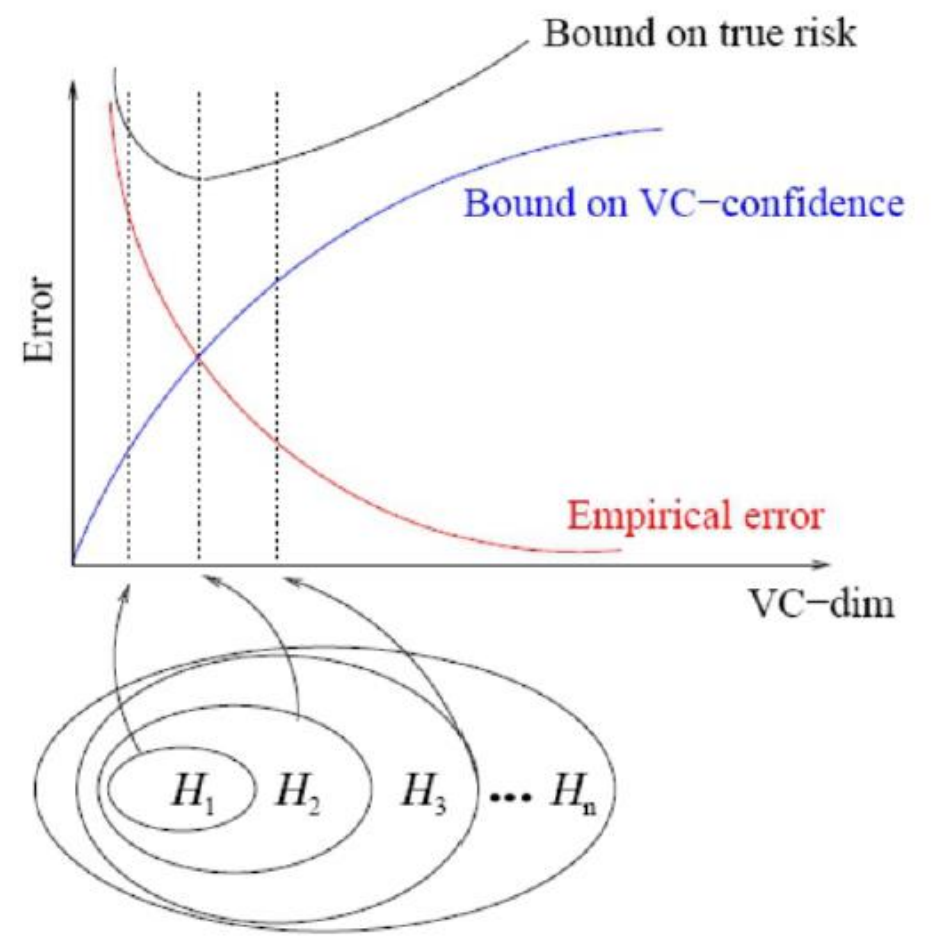
\includegraphics[width=0.5\textwidth]{./notes/immagini/l5-srm.png}
\caption{Structural Risk Minimization}
\end{figure}

% !TEX encoding = UTF-8
% !TEX program = pdflatex
% !TEX root = AALP.tex
% !TEX spellcheck = it-IT

% 20 Ottobre 2016
% \section sistemi di tipi
% \subsubsection Teorema di Preservazione (Subject reduction)

% Dimostrazione del lemma di sostituzione (spostata al posto corretto in lezione5)

\subsubsection{Corollario di Subject-reduction}

\begin{center}
	Se $\emptyset \vdash M : T$ e $M \rightarrow^* M'$, allora $\emptyset \vdash M' : T$
\end{center}

\paragraph{Dimostrazione}

La dimostrazione viene fatta per induzione sul numero di passi che da $M$ portano ad $M'$.

Il caso base è quello con il cammino di lunghezza 0, ovvero quando $M = M'$ e la tesi è trivialmente vera.

Nel caso induttivo ho che $M \rightarrow^{*}_k M_1 \rightarrow M'$, pertanto per ipotesi induttiva ho che $\emptyset \vdash M_1 : T$. 

Ho poi che $M_1 \rightarrow M'$ e quindi posso applicare subject-reduction per ottenere che $\emptyset \vdash M' : T$.

\subsubsection{Teorema di Safety - Completo}

\begin{center}
	Se $\emptyset \vdash M : T $ e $M \rightarrow^* M'$ e $M' \not\rightarrow$, allora $M'$ è un valore.
\end{center}

\paragraph{Dimostrazione}

Alle due ipotesi posso applicare il corollario di subject-reduction, ottenendo che $\emptyset \vdash M' : T$.

Per il teorema di progressione ho poi che $M'$ è un valore oppure $M'$ fa un passo e va in $M''$, ma per ipotesi $M'$ non fa un passo e quindi $M'$ è per forza un valore.

\subsection{Esercizio sul typing}

Da notare che nel contesto iniziale non servono giudizi di tipo perché tutte le variabili che compaiono sono all'interno delle funzioni e che, non essendoci informazioni sui tipi, questi sono ignoti e pertanto è necessario fare anche inferenza durante la risoluzione dell'albero.

\begin{prooftree}	
	
	% App-1
	\AxiomC{$\checkmark$ $\textbf{\textit{T}} = \textbf{\textit{T}}_1 \rightarrow \textit{\textbf{T}}_3$}
	\LeftLabel{(\textsc{Var})}
	\UnaryInfC{$y : T, x : T' \vdash y : T_1 \rightarrow T_3$}
	
	% App-2
	\AxiomC{*}
	\LeftLabel{\textsc{(If)}}
	\UnaryInfC{$y : \textbf{\textit{T}}_1\rightarrow \textbf{\textit{T}}_3, x:T' \vdash \text{if true then }x \text{ else }y \: x : T_1$}
	\LeftLabel{\textsc{(App)}}
	\BinaryInfC{$y : T, x: T' \vdash y \: (\text{if true then }x \text{ else }y \: x) : \: T_3$}
	
	\LeftLabel{\textsc{(Fun)}}
	\UnaryInfC{$y : T \vdash \fn x : \textbf{\textit{T'}} . (y \: (\text{if true then }x \text{ else }y \: x)) : \textbf{\textit{T}}_2 = \textbf{\textit{T'}} \rightarrow \textbf{\textit{T}}_3$}
	
	\LeftLabel{\textsc{(Fun)}}
	\UnaryInfC{$\emptyset \vdash \fn y : \textbf{\textit{T}} . \fn x : T' . (y \: (\text{if true then }x \text{ else }x \: y)) : \textbf{\textit{T}} \rightarrow \textbf{\textit{T}}_2$} % T' \rightarrow ?
\end{prooftree}

\noindent Dal ramo sinistro di \textsc{(App)} riesco a chiudere con $T = T_1 \rightarrow T_3$ e quindi riporto l'informazione anche sul ramo destro.
La derivazione continua applicando \textsc{(IfThenElse)} e con $\Gamma = y:T_1 \rightarrow T_3, x:T'$:

\begin{prooftree}
	%if 1
	\AxiomC{$\checkmark$}
	\LeftLabel{\textsc{(True)}}
	\UnaryInfC{$\Gamma \vdash \true : \Bool$}
	
	%if 2
	\AxiomC{$\checkmark$  $\textbf{\textit{T}}_1 = \textbf{\textit{T'}}$}
	\LeftLabel{\textsc{(Var)}}
	\UnaryInfC{$y: T_1 \rightarrow T_3, x:T' \vdash x : T_1$}
	
	%if 3
	\AxiomC{**}
	\LeftLabel{\textsc{(App)}}
	\UnaryInfC{$y : \textbf{\textit{T'}} \rightarrow T_3, x:T' \vdash y \: x : \textbf{\textit{T'}}$}
	% per quello che ho scoperto 
	\UnaryInfC{$y : T_1 \rightarrow T_3, x:T' \vdash y \: x : T_1$}
	\LeftLabel{\textsc{(If)}}
	\TrinaryInfC{(*)$\Gamma \vdash \text{if true then }x \text{ else }y \: x : T_1$}
\end{prooftree}

\noindent Dal ramo centrale della regola \textsc{(IfThenElse)} scopro che $T_1 = T'$ e quindi aggiorno il ramo destro e il contesto, che ora è  $\Gamma = y:T' \rightarrow T_3, x:T'$.

\begin{prooftree}
	\AxiomC{$\checkmark$}
	\LeftLabel{\textsc{(Var)}}
	\UnaryInfC{$y:T' \rightarrow T_3 , x:T' \vdash y : T_4 \rightarrow T'$}
	
	\AxiomC{$\checkmark$}
	\LeftLabel{\textsc{(Var)}}
	\UnaryInfC{$y : T' \rightarrow T_3 , x :T'\vdash x : T_4$}
	
	\LeftLabel{\textsc{(App)}}
	\BinaryInfC{(**)$\Gamma \vdash y \: x : T'$}
\end{prooftree}

\noindent Da quest'ultimo albero trovo che $T' = T_4 = T_3$. Andando a sostituire il tutto trovo che:

\begin{itemize}
	\item $y : T' \rightarrow T'$
	\item $x : T'$
	\item $T_2 = T' \rightarrow T_3 = T' \rightarrow T'$
	\item $T = T_1 \rightarrow T_3 = T' \rightarrow T'$
	\item Il tipo del programma è quindi $(T' \rightarrow T') \rightarrow (T' \rightarrow T')$
\end{itemize}

\chapter{Estensioni del linguaggio funzionale}

\section{Unit}

Nei linguaggi funzionali, ogni funzione deve ritornare sempre un valore, tuttavia può capitare che delle funzioni non debbano ritornare un valore. In questo caso viene ritornato il tipo \text{Unit} che può assumere l'\textbf{unico} \textbf{valore} \texttt{()} o \text{unit}.

Ad esempio la funzione \texttt{print} in Scala ritorna un valore di questo tipo:

\begin{lstlisting}[language=Scala]
def print( x: Any) : Unit = {...}
\end{lstlisting}

\noindent allo stesso modo anche l'assegnamento in Scala ritorna un valore \text{Unit} mentre in C/C++ viene solitamente ritornato il valore assegnato (per concatenare le operazioni di assegnamento).

Aggiungere \text{Unit} al linguaggio vuol dire estendere la definizione:

\begin{align*}
	M &::= \ldots \: | \: \text{unit} \: | \: \ldots \\
	v &::= \ldots \: | \: \text{unit} \: | \: \ldots \\
	T &::= \ldots \: | \: \text{Unit} \: | \: \ldots 
\end{align*}

\noindent e allo stesso modo serve una regola di tipo:

\begin{prooftree}
	\AxiomC{}
	\LL{Unit}
	\UnaryInfC{$\Gamma \vdash \text{unit : Unit}$}
\end{prooftree}

\noindent La killer-feature del tipo \text{Unit} è la possibilità di implementare il call-by-name utilizzando il call-by-value.

Ad esempio, tornano alle nostre asserzioni in Scala

\begin{lstlisting}[language=Scala, caption=Version ``standard'' delle asserzioni]
var assEnabled = true
...
def assert(pred : Bool) = 
	if (assEnabled && !pred)
		throw Exc
...

assert(saldoConto() > 0)
\end{lstlisting}


\noindent possiamo utilizzare \text{Unit} per far funzionare il codice precedente come se fosse call-by-name ma senza specificarlo:

\begin{lstlisting}[language=Scala, caption=Version ``standard'' delle asserzioni]
var assEnabled = true
...
def assert(pred : Unit => Bool) = 
	if (assEnabled && pred() == false) /** l'invocazione con () passa Unit*/
		throw Exc
...
assert(fn x:Unit . (saldoConto() > 0) ) /** pseudo scala */
assert( () =>  (saldoConto() > 0) ) /** sintassi corretta (la funzione anonima non ha parametri) */
\end{lstlisting}

\noindent In questo caso con la sintassi call-by-value viene calcolato il valore del parametro, ma in questo caso il parametro è una funzione che è già un valore.
Quindi, se le asserzioni sono disabilitate, alla chiamata della funzione \texttt{assert} non viene chiamata la funzione \texttt{saldoConto()} perché la funzione è già un valore.

Per riportare la stessa cosa nel nostro linguaggio funzionale con il call-by-value:

$$
\fn x:T.M \: N \rightsquigarrow \: \big(\fn y : \text{Unit} \rightarrow T . M\{x := y \: \text{unit}\} \big) \:\:  \big(\fn z : \text{Unit} . N \big)
$$

\subsection{Implementazione del while}

Vogliamo definire una funzione che si comporta come il while in Scala.

\begin{lstlisting}[language=Scala, caption=I parametri devono essere dichiarati come call-by-name oppure  ]
def WHILE(cond : =>Bool , command : =>Unit ) : Unit = 
	if (cond == false ) () /** In scala il return è opzionale, () è il valore di Unit*/
	else {
		command
		WHILE(cond, command)
	}

/** Uso della funzione */
var a = 0
WHILE(a < 4 , {print(a); a=a+1})
\end{lstlisting}

\noindent Dato che sono in call-by-value i parametri vengono valutati prima di invocare per la prima volta il while, quindi o li passo per by-name oppure li passo utilizzando una funzione. 
Questo perché sia il codice del corpo che la condizione devono poi essere rieseguiti (valutati) nelle successive iterazioni. 



\chapter{Il modello lineare nei parametri}

\textbf{Problema di riferimento:} come il prezzo influenza il consumo di
gas? Si hanno a disposizione le informazioni relative alla domanda di
gas e al prezzo dello stesso per 20 città in Texas.

Si vuole riuscire a capire se c'è una correlazione tra le due cose.

\begin{figure}[htbp]
	\centering
	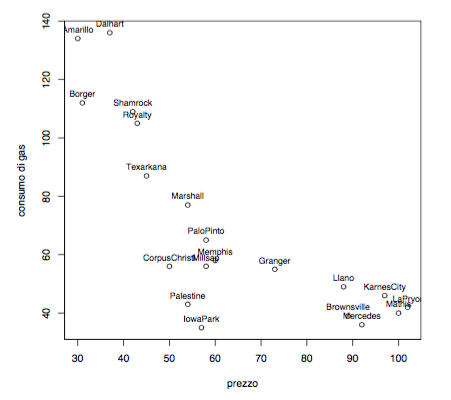
\includegraphics[width=.5\textwidth]{./notes/immagini/l7-fig1.png}
\end{figure}

\section{Un primo modello lineare}\label{un-primo-modello-lineare}

Ipotizzando che ci sia una relazione lineare è possibile utilizzare il
modello del capitolo precedente:

$$
y = \alpha + \beta x + \epsilon
$$

$$
\hat{\beta} = \frac{\cov(X,Y)}{\var(X)} \qquad \hat{\alpha} = \bar{y} - \hat{\beta}\bar{x}
$$

Utilizzando l'ambiente R si ottengono delle informazioni relative all
modello ottenuto:

\begin{verbatim}
lm(formula = gas ~ prezzo)
Residuals:
    Min      1Q  Median      3Q     Max
-40.625 -10.719  -1.136  14.073  38.292
Coefficients:
            Estimate Std. Error t value Pr(>|t|)
(Intercept)  138.561     13.552  10.225 6.34e-09 ***
prezzo        -1.104      0.202  -5.467 3.42e-05 ***
---
Signif. codes:  0 ‘***’ 0.001 ‘**’ 0.01 ‘*’ 0.05 ‘.’ 0.1 ‘ ’ 1
Residual standard error: 20.86 on 18 degrees of freedom
Multiple R-Squared: 0.6241,     Adjusted R-squared: 0.6033
F-statistic: 29.89 on 1 and 18 DF,  p-value: 3.417e-05
\end{verbatim}

Dai dati si può notare che l'indice $ R^2 $ è uguale a 0.62, il che indica un buon andamento lineare.
Inoltre come \textit{p-value} si ottiene un valore molto basso, il che porta a rifiutare l'ipotesi nulla.

Tracciando però i grafici dei residui è possibile osservare c'è una componente indipendente che non è lineare.

\begin{figure}[htbp]
	\centering
	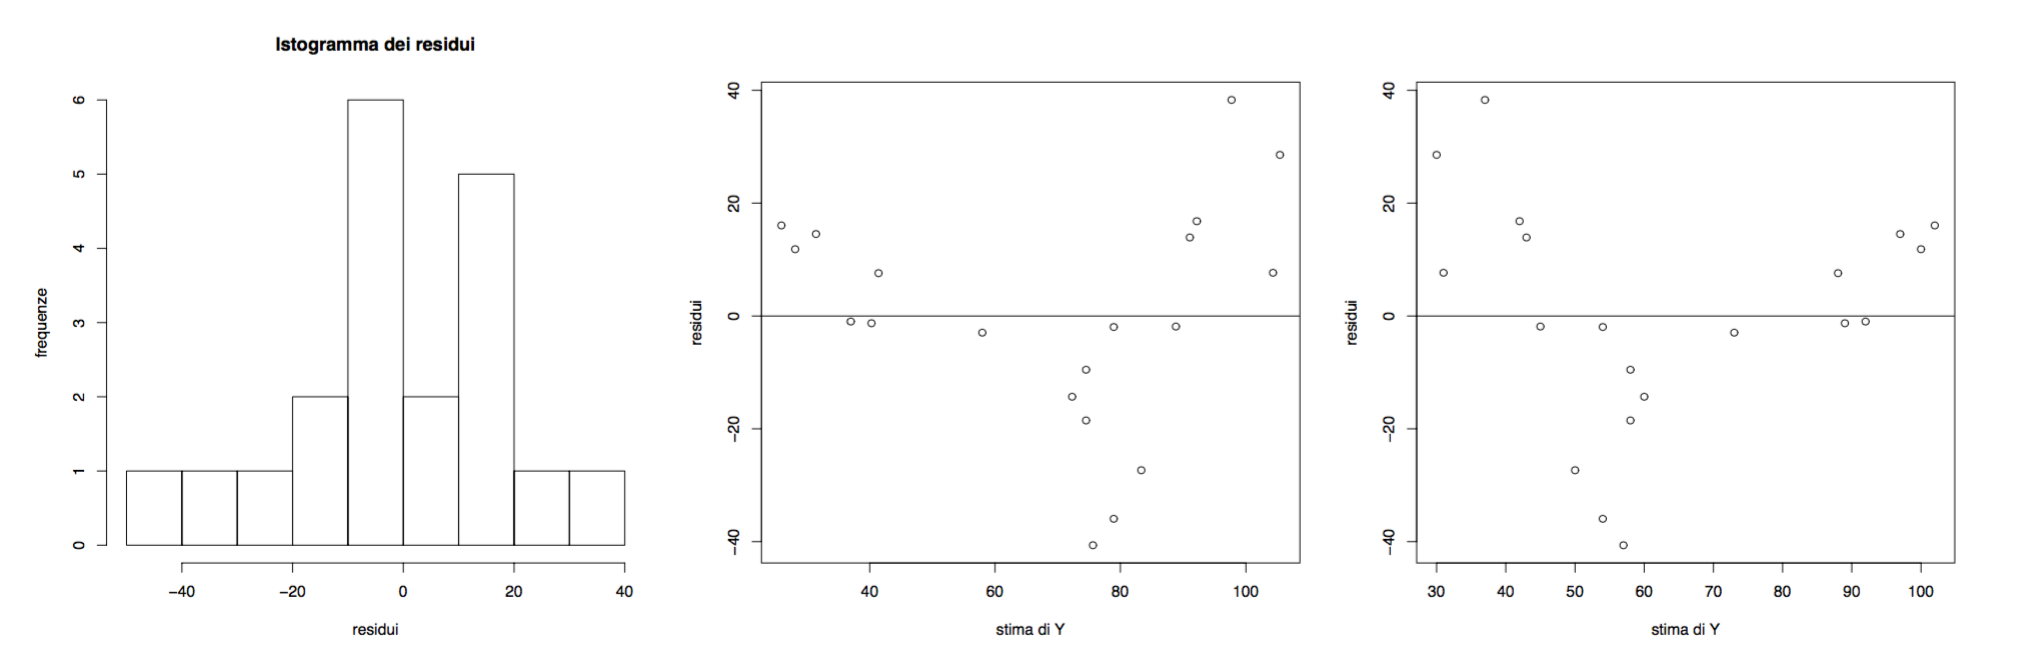
\includegraphics[width=1\textwidth]{./notes/immagini/l7-fig2.png}
	\caption{Tracciamento dei residui per il primo modello. \`{E} possibile notare la presenza di indipendente.}
\end{figure}

\section{Considerazioni sul problema e un secondo modello}\label{considerazioni-sul-problema-e-un-secondo-modello}

Considerando il problema modellato è possibile fare alcune osservazioni:

\begin{itemize}
	\item il consumatore potrebbe destinare solamente un determinato budget $ \kappa $ per l'acquisto del gas, ovvero $ x \cdot y = \kappa $.
	\item è ragionevole pensare che il consumatore debba consumare una quantità minima di gas $ \gamma $
	\item essendo il mercato del gas regolamentato, c'è un prezzo minimo di $ 7 $ centesimi al metro cubo sotto il quale non è possibile vendere il gas.
\end{itemize}

Tenendo in considerazione quanto elencato si arriva ad avere l'equazione:

$$
(x-7)(y-\gamma) = \kappa
$$

la quale può essere riscritta in un modo più simile a quella del modello lineare

$$
y = \gamma + \kappa \cdot \frac{1}{x-7}
$$

e sostituendo la variabile \textit{x} con $ z = \frac{1}{x-7} $, si ottiene proprio la stessa equazione la quale permette di calcolare la retta ai minimi quadrati.

Questo è possibile perché quello che finora è stato chiamato modello lineare è un caso particolare dei \textbf{modelli lineari nei parametri}. Ovvero la limitazione data dalla linearità non riguarda le variabili, ma riguarda solamente i \textbf{parametri} del modello.

Quando viene utilizzato il metodo dei minimi quadrati con questi modelli è necessario tenere in considerazione le trasformazioni che vengono fatte alle variabili, perché i valori calcolati ai minimi quadrati riguardano le variabili trasformate e non quelle di partenza, è necessario quindi \textbf{scalare} in modo opportuno i valori\footnote{Se viene scalata solamente la $ x $ non c'è questo problema perché i minimi quadrati considerano solamente le distanze rispetto l'asse $ y $.}.

La formulazione più generale del modello lineare è quindi

$$
g(y) = \alpha + \beta h(x) + \epsilon
$$

Il modello ottenuto per la nuova formulazione è:
\begin{verbatim}
lm(formula = gas ~ I(1/(prezzo - 7)))
Residuals:
Min    1Q  Median  3Q    Max
-29.617 -4.574 2.394 7.800 30.917
Coefficients:
Estimate Std. Error t value Pr(>|t|) 
(Intercept) 3.918 8.376 0.468 0.646
I(1/(prezzo - 7)) 3034.938 357.037 8.500 1.02e-07 *** 
---
Signif. codes: 0 ‘***’ 0.001 ‘**’ 0.01 ‘*’ 0.05 ‘.’ 0.1 ‘ ’ 1
Residual standard error: 15.19 on 18 degrees of freedom 
Multiple R-Squared: 0.8006, Adjusted R-squared: 0.7895 
F-statistic: 72.26 on 1 and 18 DF, p-value: 1.022e-07
\end{verbatim}

ovvero la retta

$$
y = 3.918 + 3034.938 \cdot \frac{1}{x-7}
$$

\begin{figure}[htbp]
	\centering
	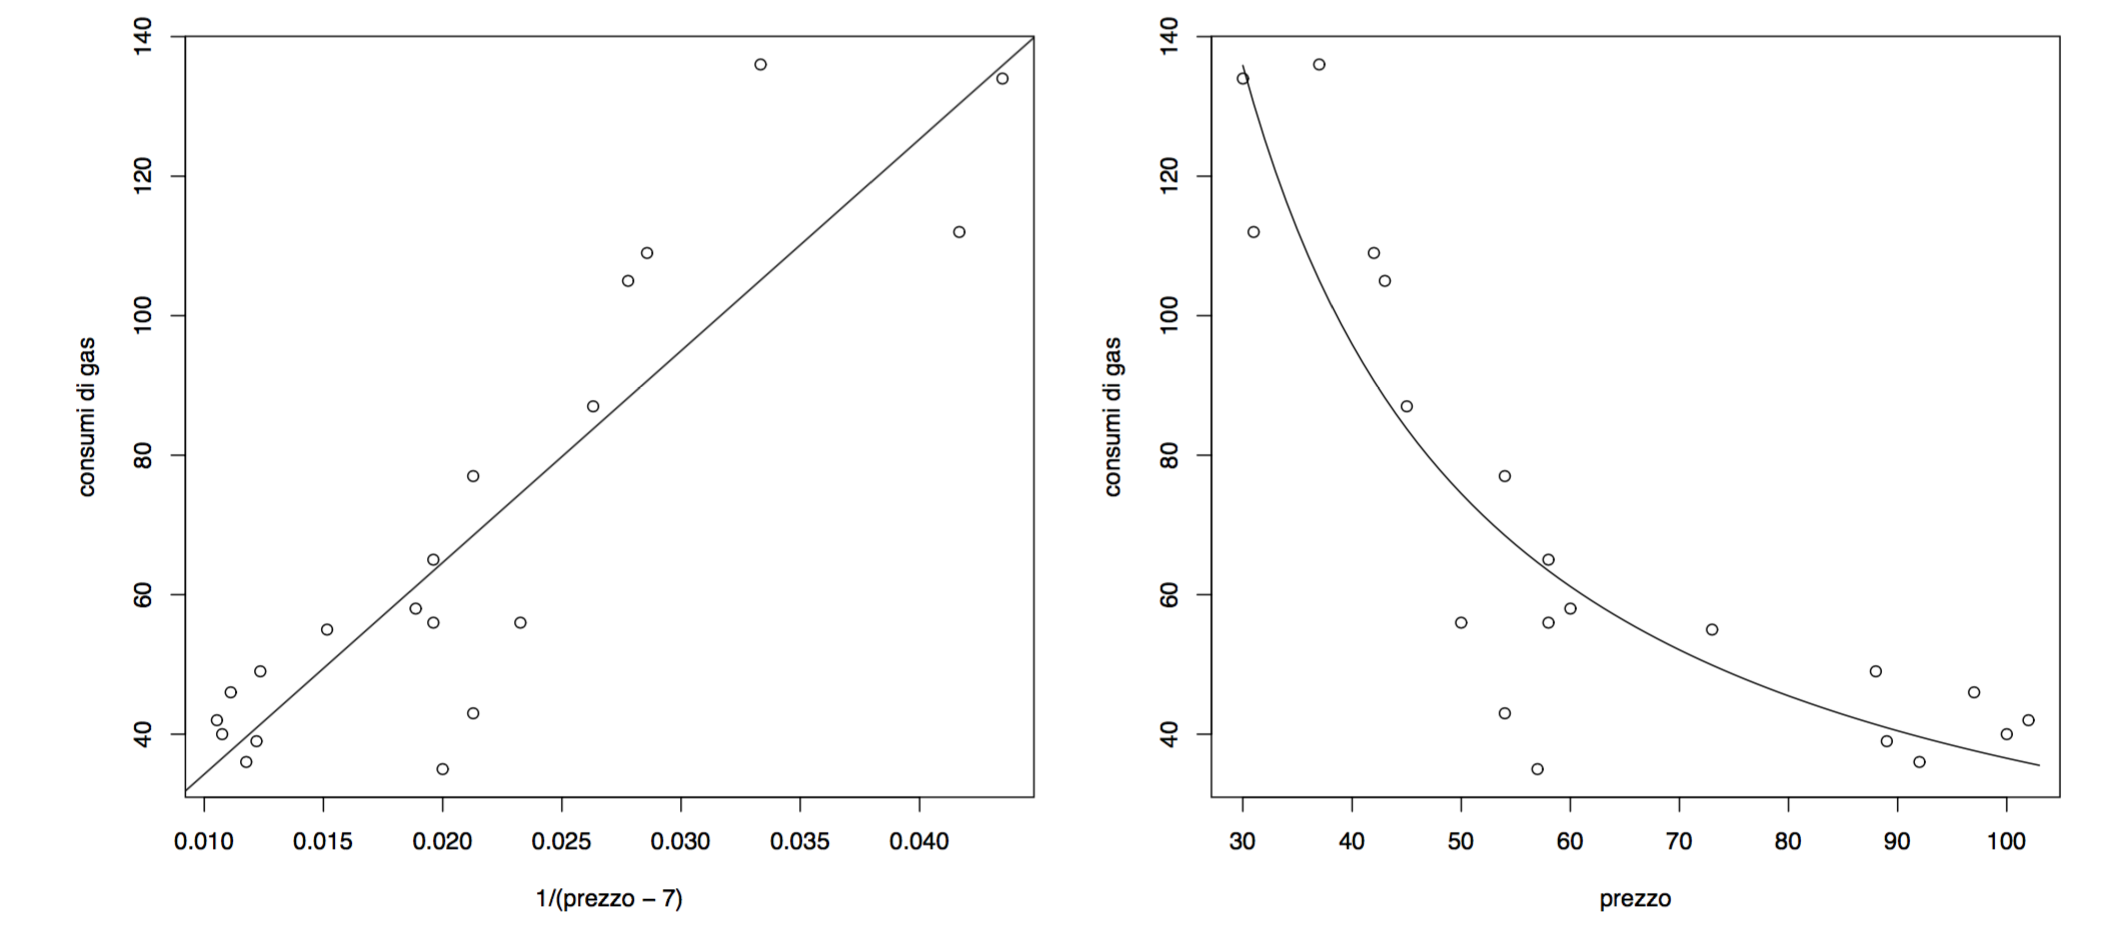
\includegraphics[width=1.1\textwidth]{./notes/immagini/l7-fig3.png}
	\caption{A destra la retta rispetto $ z $. A sinistra il modello lineare tracciato rispetto $ x $.}
\end{figure}

Dai dati del nuovo modello è possibile osservare che la varianza residua (\texttt{Residual standard error} elevato al quadrato) è passata da circa 391 a circa 207, ovvero il quadrato degli errori di previsione è stato ridotto di quasi il $ 50\% $.
Lo stesso effetto può essere visto utilizzando $ R^2 $ che da 0.6241 passa a 0.8006.

\begin{figure}[htbp]
	\centering
	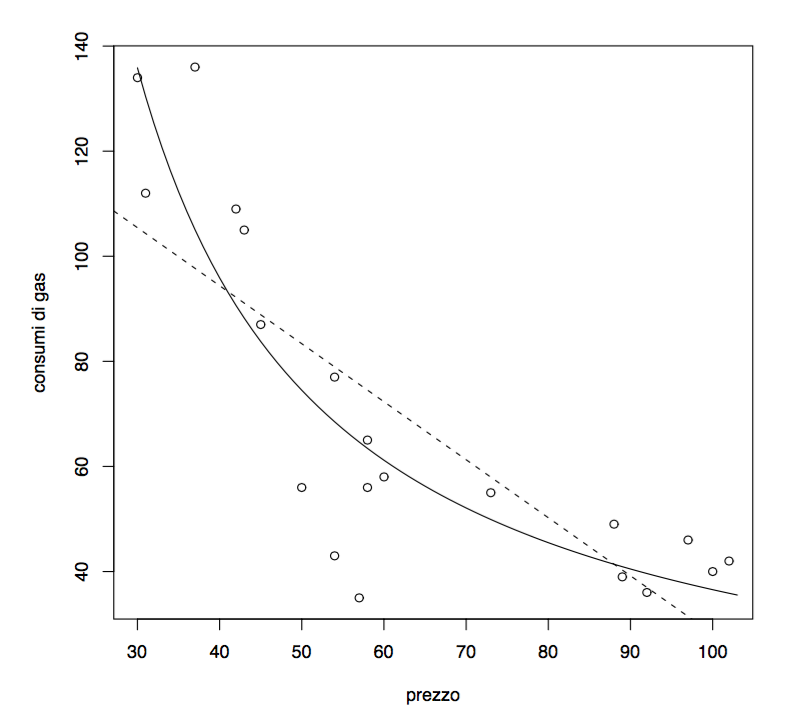
\includegraphics[width=.6\textwidth]{./notes/immagini/l7-fig4.png}
	\caption{Confronto grafico tra i due modelli.}
\end{figure}

\FloatBarrier
\section{Modello lineare con trasformate}\label{modello-lineare-con-trasformate}

\textit{Cambia il dataset di riferimento}, si vuole controllare se il reddito nazionale influisce sulla speranza di vita media dello stato. 

\begin{figure}[htbp]
	\centering
	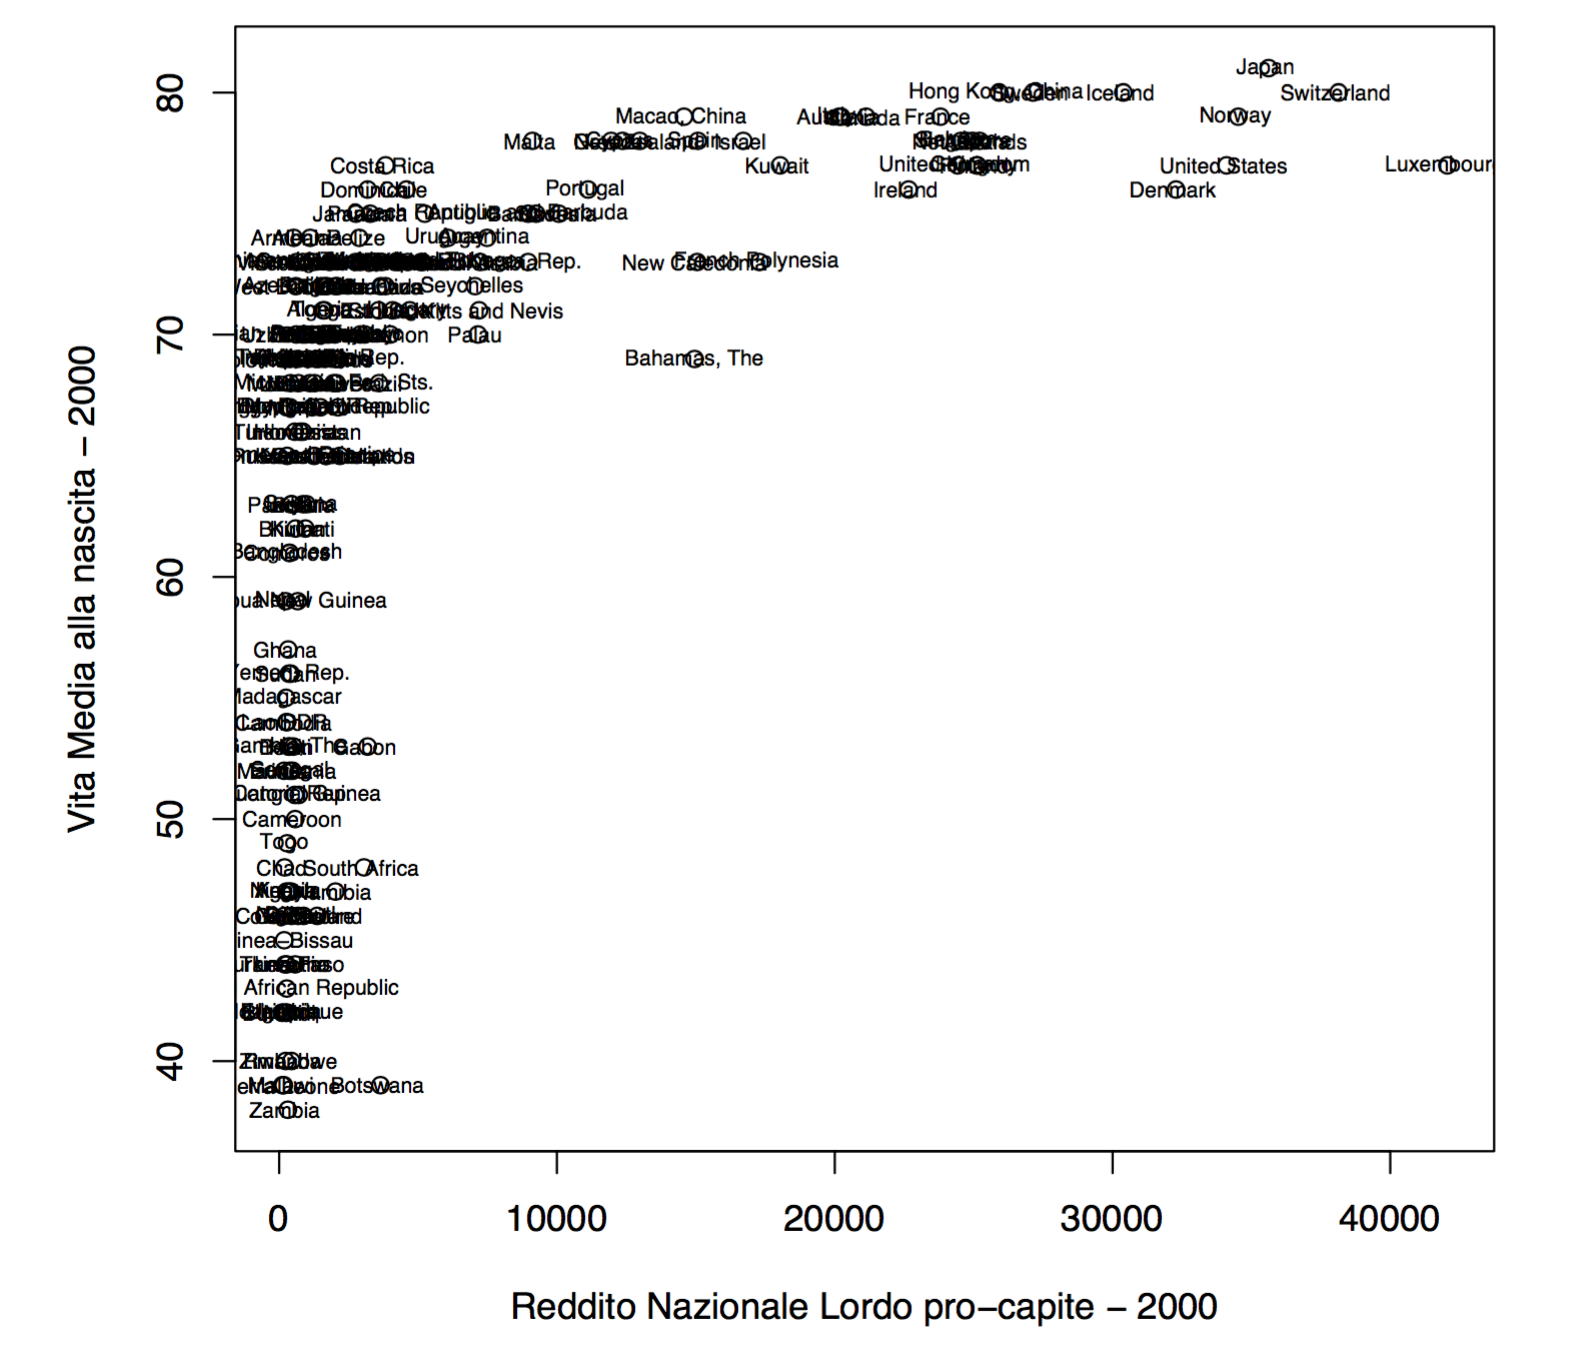
\includegraphics[width=.7\textwidth]{./notes/immagini/l7-fig5.png}
	\caption{Dataset - GNI - ELF}
\end{figure}

La prima cosa da fare è osservare come si comporta il modello lineare senza trasformazioni:

\begin{verbatim}
	lm(formula = elf ~ GNIpc)
	Residuals:
	Min    1Q  Median  3Q    Max
	-24.924 -7.512 4.119 7.431 12.948
	Coefficients:
	Estimate Std. Error t value Pr(>|t|)
	(Intercept) 6.133e+01 8.967e-01 68.390 < 2e-16 ***
	GNIpc 7.115e-04 8.230e-05 8.645 3.76e-15 ***
	---
	Signif. codes: 0 ‘***’ 0.001 ‘**’ 0.01 ‘*’ 0.05 ‘.’ 0.1 ‘ ’ 1
	Residual standard error: 9.903 on 171 degrees of freedom 
	Multiple R-Squared: 0.3041, Adjusted R-squared: 0.3 
	F-statistic: 74.73 on 1 and 171 DF, p-value: 3.757e-15
\end{verbatim}

Si può notare come l'indice $ R^2 $ sia molto basso (0.3041), ma risulta essere molto significativo perché, per il \textit{p-value} ottenuto sia ha che è improbabile che valga l'ipotesi nulla.

Tracciando il modello e il grafico dei residui è possibile notare che
\begin{itemize}
	\item La retta ottenuta non curva abbastanza e quindi non si adatta bene ai dati
	\item Il modello prevede una vita media che può essere maggiore di 90 anni, il che è abbastanza improbabile.
\end{itemize}

\begin{figure}[htbp]
	\centering
	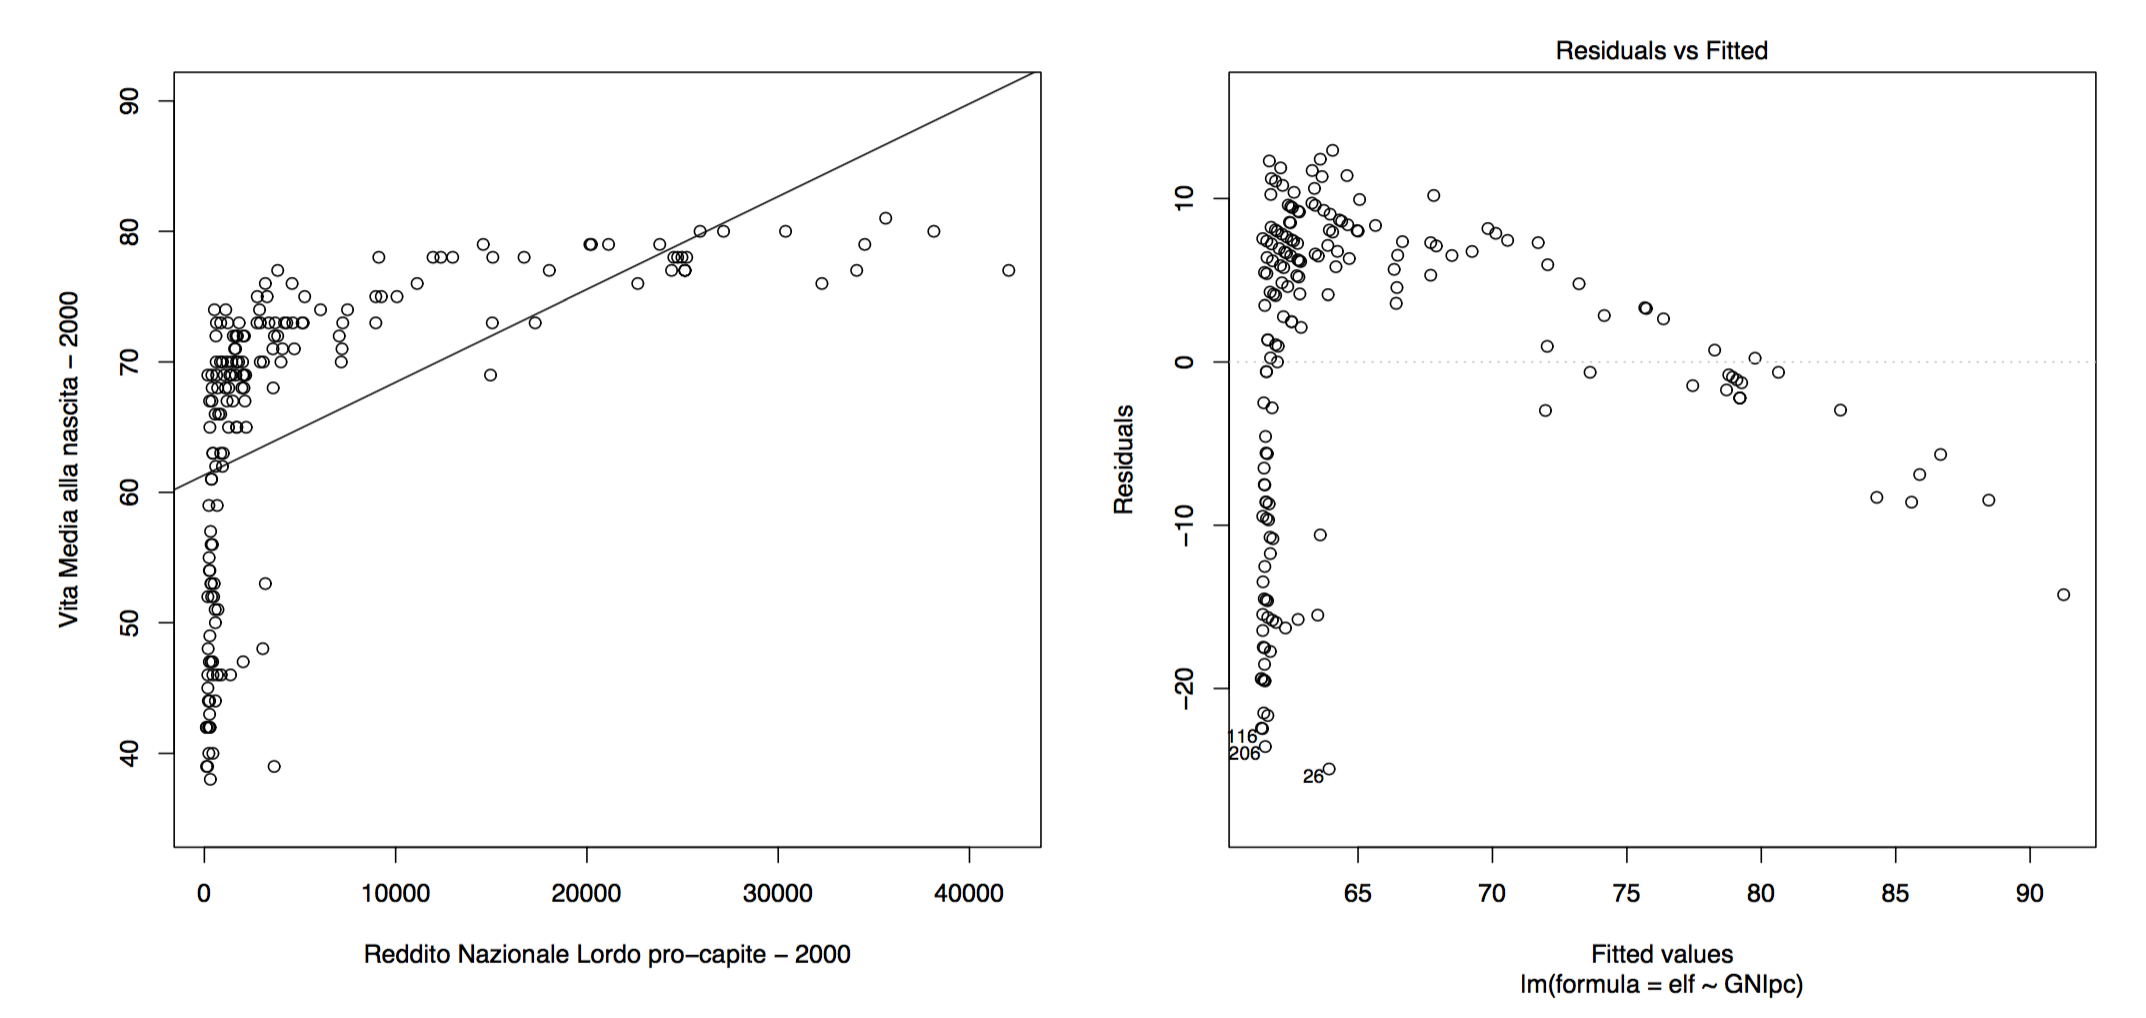
\includegraphics[width=.9\textwidth]{./notes/immagini/l7-fig6.png}
	\caption{Primo modello e residui ottenuti}
\end{figure}

Per adattare meglio la curva è possibile utilizzare la scala logaritmica per l'asse delle \textit{x}. In questo modo, al crescere del reddito viene dato via via meno peso.
Inoltre, rappresentando graficamente questa trasformazioni si ottiene una nuvola di punti più simile ad una retta.

\begin{figure}[htbp]
	\centering
	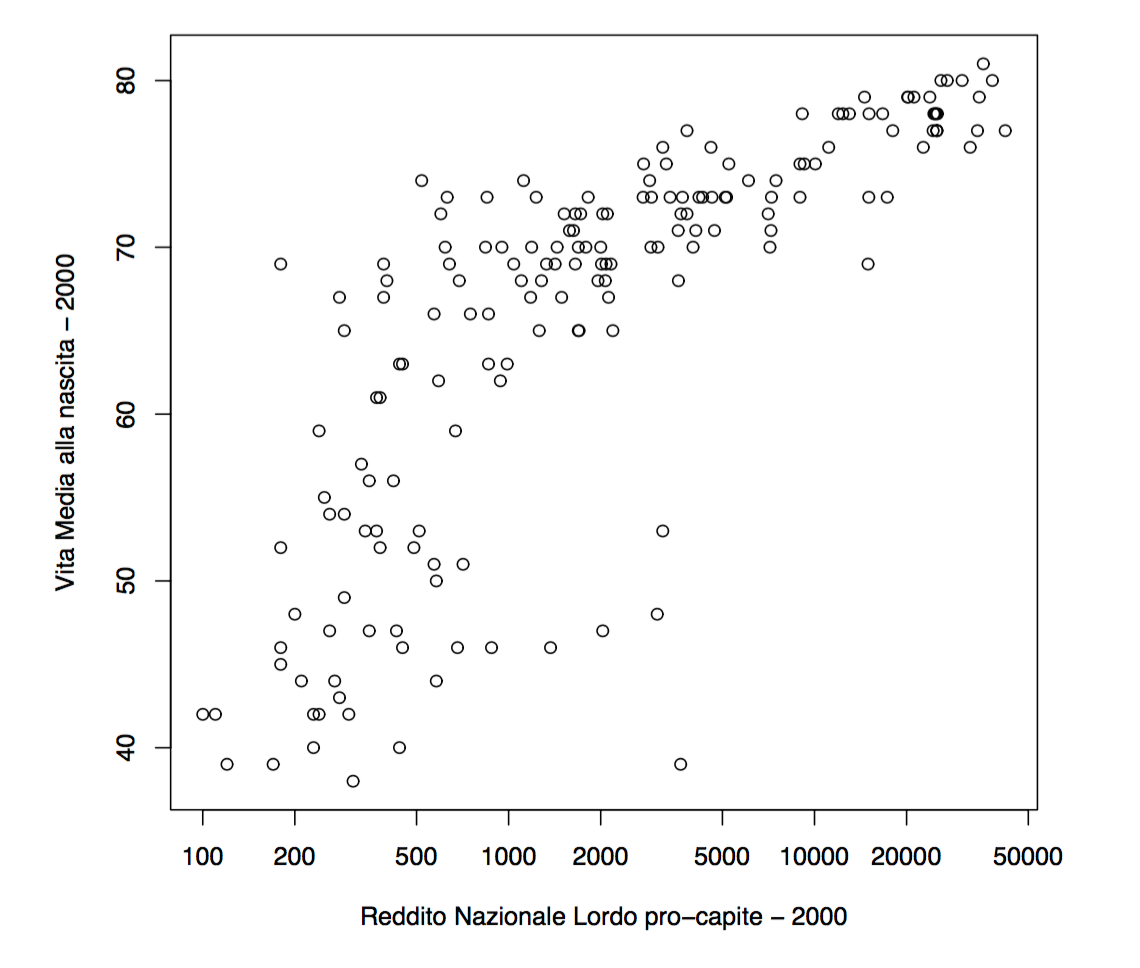
\includegraphics[width=.6\textwidth]{./notes/immagini/l7-fig7.png}
	\caption{Grafico che utilizza la scala logaritmica per i valori delle $ x $. L'asse è comunque etichettato con i valori originali.}
\end{figure}

Il modello diventa quindi

$$
(\text{vita media alla nascita}) = \alpha + \beta \log(\text{reddito nazionale pro capite})
$$

\begin{verbatim}
lm(formula = elf ~ I(logGDP), data = elf.data)
Residuals:
Min     1Q   Median   3Q     Max
-29.6591 -2.9511 0.7906 5.1050 17.4844
Coefficients:
Estimate Std. Error t value Pr(>|t|)
(Intercept) 22.6701 2.8447 7.969 2.02e-13 *** 
I(logGDP) 5.6767 0.3677 15.438 < 2e-16 ***
---
Signif. codes: 0 ‘***’ 0.001 ‘**’ 0.01 ‘*’ 0.05 ‘.’ 0.1 ‘ ’ 1
Residual standard error: 7.674 on 174 degrees of freedom 
Multiple R-Squared: 0.578, Adjusted R-squared: 0.5756 
F-statistic: 238.3 on 1 and 174 DF, p-value: < 2.2e-16
\end{verbatim}

Con questo secondo modello si ottiene un indice $ R^2 $ doppio rispetto al precedente e questo può essere osservato anche nella rappresentazione grafica del nuovo modello.

\begin{figure}[htbp]
	\centering
	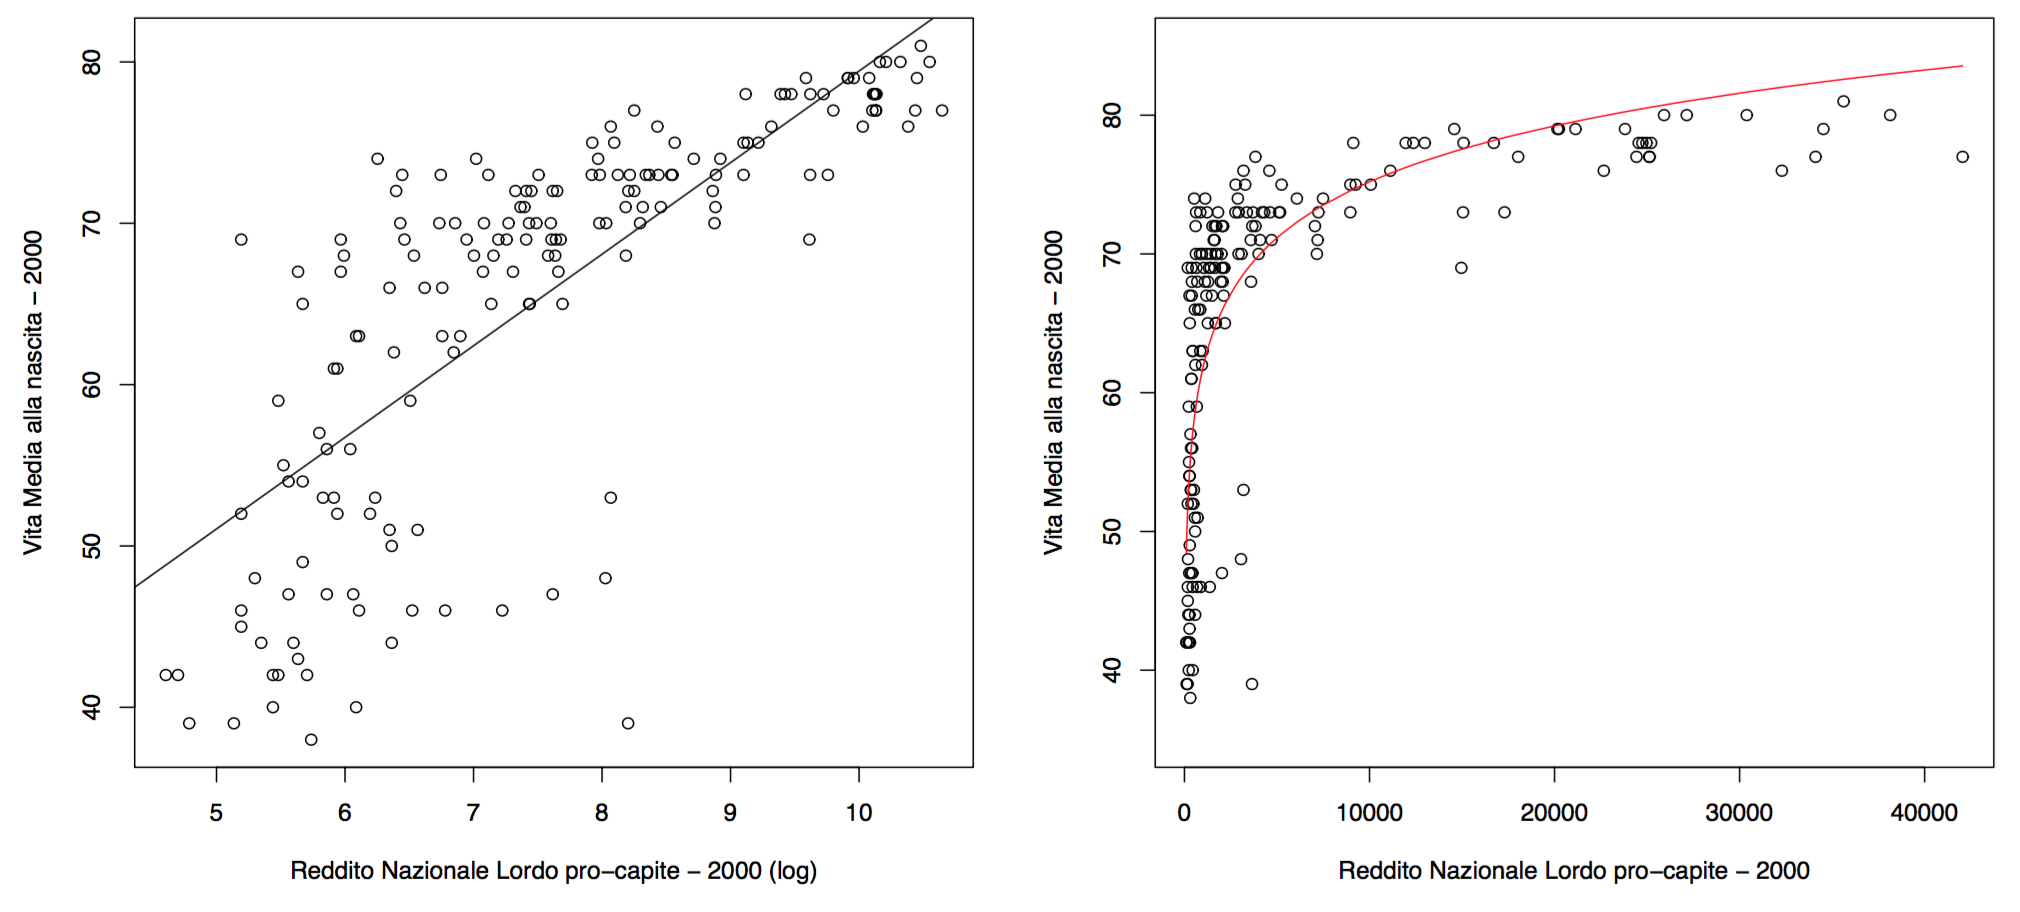
\includegraphics[width=.9\textwidth]{./notes/immagini/l7-fig8.png}
	\caption{Secondo modello: a sinistra con la scala logaritmica, a destra normale.}
\end{figure}

C'è però ancora un problema che riguarda i valori estremi che non vengono approssimati bene dalla curva e lo si può notare anche dai residui.

\begin{figure}[htbp]
	\centering
	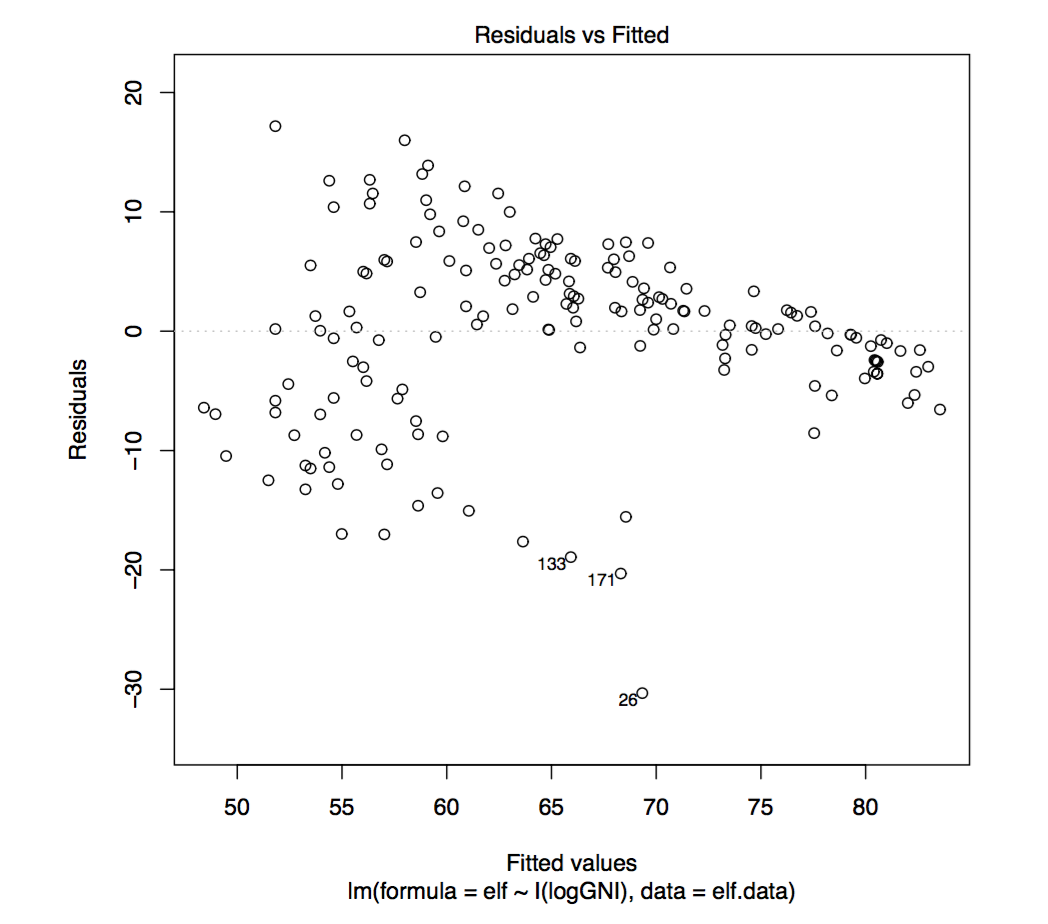
\includegraphics[width=.6\textwidth]{./notes/immagini/l7-fig9.png}
	\caption{Residui per il secondo modello }
\end{figure}

Un'ulteriore modifica può essere quella di trasformare anche la variabile risposta, elevandola alla quinta, in modo da dare maggior peso ai valori maggiori.

Il modello ottenuto è quindi dato da

$$
(\text{vita media alla nascita})^5 = \alpha + \beta \log(\text{reddito nazionale pro capite}) + \epsilon
$$

Da notare che con questa formulazione le ipotesi sugli errori (media nulla, varianza costante, distribuzione normale, ecc.) \textbf{devono valere per gli errori su scala trasformata}.

Una volta calcolato il modello si ottiene

\begin{verbatim}
lm(formula = elf.5 ~ logGNI, data = elf.data)
Residuals:
Min        1Q        Median    3Q       Max
-1.801e+09 -2.817e+08 7.965e+06 3.036e+08 1.334e+09
Coefficients:
Estimate Std. Error t value Pr(>|t|) 
(Intercept) -2.345e+09 1.832e+08 -12.80 <2e-16 *** 
logGNI 5.164e+08 2.376e+07 21.73 <2e-16 ***
---
Signif. codes: 0 ‘***’ 0.001 ‘**’ 0.01 ‘*’ 0.05 ‘.’ 0.1 ‘ ’ 1
Residual standard error: 4.89e+08 on 171 degrees of freedom 
Multiple R-Squared: 0.7341, Adjusted R-squared: 0.7326 
F-statistic: 472.2 on 1 and 171 DF, p-value: < 2.2e-16
\end{verbatim}

\begin{figure}[htbp]
	\centering
	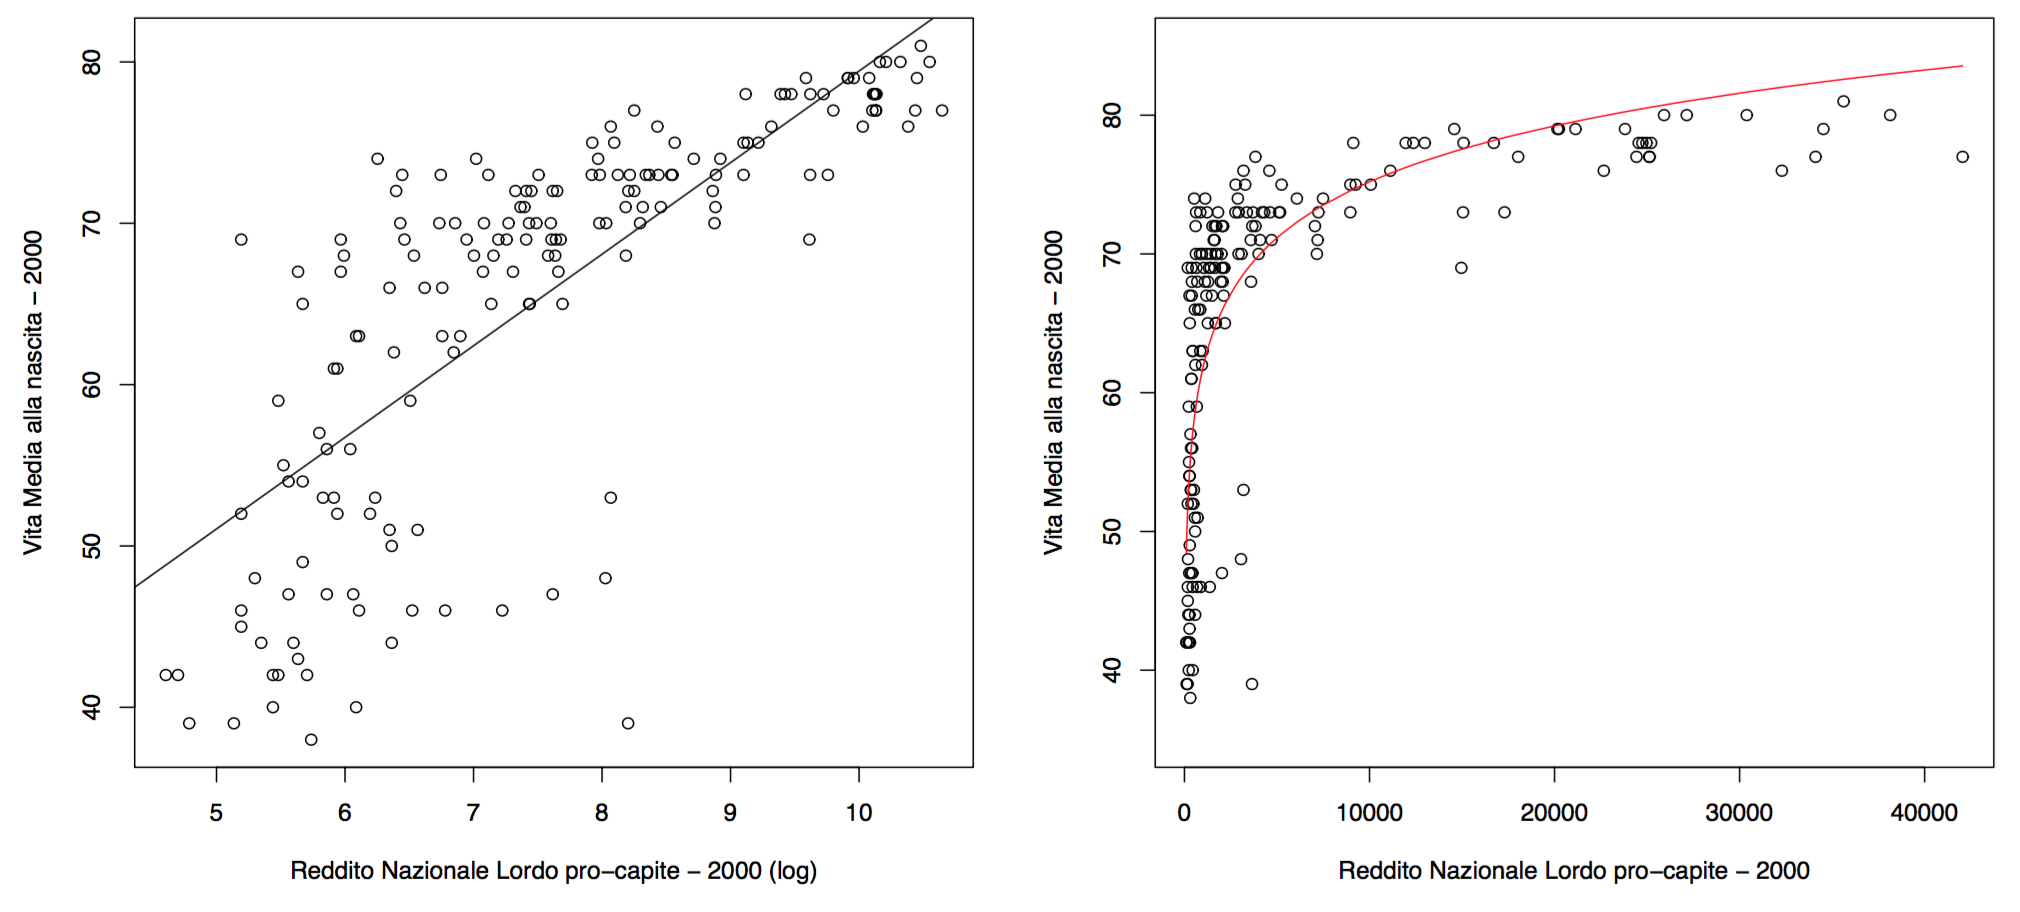
\includegraphics[width=.9\textwidth]{./notes/immagini/l7-fig8.png}
	\caption{Terzo modello: a sinistra con la scala originale e a destra i residui.}
\end{figure}

L'indice $ R^2 $ ottenuto fa riferimento ai residui calcolati sulla scala trasformata, quindi per avere un'indice di adattamento dei dati è possibile utilizzare la media dei quadrati dei residui per la variabile originale:

$$
\frac{1}{n}\sum\limits_{i=1}^n \bigg[ \big(\text{vita media alla nascita}\big)_i - \sqrt[5]{\big(\alpha + \beta \log(\text{reddito nazionale pro capite})_i\big)}\bigg]^2
$$

Calcolando questo valore si ottiene 55.08, mentre con il secondo modello si aveva la varianza dei residui pari a 58.89. Si ottiene quindi una riduzione del $ 6\% $ del quadrato degli errori di previsione.










% !TEX encoding = UTF-8
% !TEX program = pdflatex
% !TEX root = AALP.tex
% !TEX spellcheck = it-IT

% 27 Ottobre 2016
%\section{Estensioni del nostro linguaggio}
%\subsection{Record}
% \subsubsection{L'oggetto conto}

\section{Tipi variante}

Se i record possono essere visti come tipi congiunzione, che combinano più tipi, i tipi variante possono essere visti come disgiunzione.

Ad esempio possiamo pensare ad un contatto in una rubrica che può avere un indirizzo fisico o virtuale:

$$
< \text{fisico}: \underbrace{\{ \text{nome : String}, \text{indirizzo: String} \}}_{T_{fisico}} , \: \text{virtuale}: \underbrace{\{ \text{login : String}, \text{email : String} \}}_{T_{virt}} >= T_{ind}
$$

\noindent Un esempio di valore che ha questo tipo è:

$$
< \text{fisico} = \{ \text{nome = ``pippo''}, \text{indirizzo =  ``Via rosa''} \} >
$$

\noindent L'utilità di questi tipi si ha con l'operatore di pattern matching.
Ad esempio in Scala è possibile definire delle funzione generiche che lavorano sui tipi variante:

\begin{lstlisting}[language=Scala, caption=Utilizzo del pattern matching in Scala]
def getName(a : Tind) : String = a match{
	case <fisico = x> => x.nome
	case <virtuale = x> => x.login
	/** case <l = x> => ... da errore di compilazione! */
	/** allo stesso modo viene segnalato se il pattern non copre tutte le possibili etichette */
}

def getAll(a : List[Tind] ) : List[String] = {
	var l = new List[String]
	for (x <- a) l.add(getName(x))
}
\end{lstlisting}

\noindent Per inserire nel nostro linguaggio questi valori servono dei nuovi termini:

$$
M ::= < l = M > \vbar M \text{ match } \{\text{case }l_i = x_i => M_i \:^{i = 1\ldots n}\} \vbar \ldots
$$

\noindent Da notare che la $x_i$ che viene utilizzata nel \text{match} lega le eventuali occorrenze all'interno di $M_i$.

$$
<l_1 = 3> \text{ match } \{\text{case } l_1 = x => x+1, \ldots \} \rightarrow 3+1
$$

\noindent Più formalmente:

\begin{itemize}
	\item $fv(<l =M>) = fv(M)$
	\item $fv( M \text{ match } \{\text{case }l_i = x_i => M_i \:^{i = 1\ldots n}\}) = fv(M) \cup \bigcup_{i = 1 \ldots n}\bigg( fv(M_i) \setminus \{x_i\} \bigg) $
\end{itemize}


\noindent Servono inoltre dei nuovi valori finali e dei tipi:

$$
v ::= <l = v> \vbar \ldots \qquad T ::= < l_i : T_i \:^{i = 1 \ldots n}>
$$

\noindent La semantica operazionale viene espressa con 3 nuove regole:

\begin{itemize}
	\item Riduzione del termine interno
	\begin{prooftree}
		\AxiomC{$M \rightarrow M'$}
		\LL{Variant}
		\UnaryInfC{$<l = M> \rightarrow <l = M'>$}
	\end{prooftree}
	\item Avanzamento in un match:
	\begin{prooftree}
		\AxiomC{$M \rightarrow M'$}
		\LL{Red-Match}
		\UnaryInfC{$M \text{ match } \{\text{case } l_i = x_i => M_i \:^{i = 1 \ldots n}\} \to M' \text{ match } \{\text{case } l_i = x_i => M_i \:^{i = 1 \ldots n}\}$}
	\end{prooftree}
	\item Assioma per il match effettivo
	\begin{prooftree}
		\AxiomC{$j \in \{1 \ldots n\}$}
		\LL{Match}
		\UnaryInfC{$<l_j = v> \text{ match } \{\text{case } l_i = x_i => M_i \:^{i = 1 \ldots n}\} \rightarrow M_j\{x_j = v\}$}
	\end{prooftree}
\end{itemize}

\noindent Servono inoltre delle regole di tipo, una per l'invariante e l'altra per il match.

\begin{prooftree}
	\AxiomC{$ \Gamma \vdash M: T_j $}
	\AxiomC{$ j \in \{1 \ldots n \} $}
	\LL{Type-Variant}
	\BinaryInfC{$\Gamma \vdash <l_j = M> : <l_i : T_i \:^{i=1\ldots n}>$}
\end{prooftree}

\noindent Con questa regola posso assegnare ad un valore infiniti tipi, l'importante è che in questi infiniti tipi ci sia l'etichetta $l_j$ in modo da avere la garanzia di riuscire ad effettuare il pattern matching.

\begin{prooftree}
	\AxiomC{$\Gamma \vdash M : < l_i : T_i  \:^{i=1\ldots n}>$}
	\AxiomC{$\Gamma, x_i : T_i \vdash M_i : T \:\: \forall \: i = 1 \ldots n $}
	\LL{Type-Match}
	\BinaryInfC{$\Gamma \vdash M \text{ match }\{\text{case }l_i = x_i => M_i \:^{i=1\ldots n}\} : T$}
\end{prooftree}

\noindent Perché un match sia ben tipato è necessario che il termine $M$ sia un valore di tipo variante e che tutti i ``rami'' del match siano termini con lo stesso tipo, aggiungendo anche al contesto la sostituzione che viene effettuata quando viene applicato il match.

Se nel pattern matching ho come premessa della regola $\Gamma \vdash M : < l_i : T_i  \:^{i=1\ldots m}>$ con $m \geq n$ c'è un problema perché possono capitare delle etichette che il costrutto \text{match} non riesce a gestire. Se invece $m \leq n$ non ci sono problemi. Ma anche in questo caso, dato che ho a disposizione infiniti tipi, conviene forzare $m = n$.

Anche se non sembra questi tipi sono presenti nella maggior parte dei linguaggi main stream, solo che questi vengono nascosti da dello zucchero sintattico. Ad esempio le liste possono essere viste come un tipo variante in quanto sono o una lista vuota o la concatenazione di un elemento e un'altra lista.

$$
\text{List} = < \text{nil : Unit}, \text{cons} : (\Nat * \text{List}) >
$$

\noindent Si tratta di un tipo ricorsivo che non è supportato nella nostra grammatica, ma in altre grammatiche è possibile gestirlo.

I valori per questo tipo sono:

$$
<\text{nil } = \text{unit}>  \quad <\text{cons} = (5, <\text{nil } = \text{unit}>)>
$$

\noindent Un altro caso d'uso dei valori variante è l'analisi delle dereferenziazioni dei valori null.
Ad esempio in Java possiamo definire una variabile e assegnarle null:

\begin{lstlisting}[language=Java]
C c = null;

C find(List<C> l, C a) { ... } // se non trova ritorna null

C c = find(list, s);
// c può essere null, quindi devo controllare
// se non controllo potrei finire in un NullPointerException, anche perché il compilatore non controlla questo tipo di eccezioni
if (c != null) print(c.info());
else print("non trovato");
\end{lstlisting}

\noindent Questo approccio non è dei migliori, perché dovrebbe utilizzare le eccezioni personalizzate, ma si è visto che nessuno le usa. Con C\# si sono invece inventati i tipi \texttt{Nullable} che possono avere anche come valore \texttt{Null}, anche per i tipi primitivi.

Un'altra idea è stata quella di introdurre i tipi \texttt{!}: una classe di tipo \texttt{C!} non può assumere come valore null, in modo da sfruttare di più l'analisi statica.

Linguaggio che vai, soluzione che trovi. Altri linguaggi utilizzano i così detti \textbf{null objects}:

\begin{lstlisting}[language=Java]
class C {
	...
	String info() {...}
	...
}
class NullC extends C {
	...
	String info() {}
}
\end{lstlisting}

\noindent Così facendo c'è un metodo definito da chiamare anche sul valore null, in modo da evitare la NullPointerExcpetion.

Scala e Java8 (e Swift) implementano un'ulteriore versione, gli \textbf{option type}, ovvero un tipo variante che prevede due possibilità: c'è l'oggetto oppure non c'è.
La definizione di questo tipo è la seguente:

$$
Option[C] = < \text{none} : \text{Unit}, \text{some} : C >
$$

\noindent Il codice di prima può essere quindi riscritto come

\begin{lstlisting}[language=Scala]
...
def find(l : List[C], s : String) : Option[C] = {
	for(x <- l) 
		if (x.info() == s) return Some(x)
	return None 
}
...
find(l, "pippo") match {
	case Some(x) => print(x.info())
	case None => print("non trovato")
}
\end{lstlisting}

\noindent Si può notare come questa versione del codice è più espressiva e si riesce subito a capire che la funzione \texttt{find} può non trovare l'elemento cercato.



% !TEX encoding = UTF-8
% !TEX TS-program = pdflatex
% !TEX root = computabilità e algoritmi.tex
% !TEX spellcheck = it-IT
\chapter{Algoritmi su stringhe}\label{algoritmi-su-stringhe}

\section{Il problema del matching esatto}\label{il-problema-del-matching-esatto}

Si ha un pattern \emph{P} di lunghezza \emph{m} e un testo \emph{T} in
cui cercare il pattern di lunghezza $n \geq m$.

Un esempio di problema è la ricerca del pattern \emph{P = aba} in
\emph{T=bbabaxababay}. In questo caso ci sono 3 occorrenze del pattern,
che si sovrappongono tra loro.

Risolvere questo problema in modo efficiente è di importanza chiave dal
momento che tutti i motori di ricerca si basano sul pattern matching
esatto o approssimato. Un altro campo in cui è utile il pattern matching
è nella bioinformatica, infatti, il DNA umano può essere visto come una
stringa di 4 miliardi di caratteri.

\subsection{Notazione utilizzata}\label{notazione-utilizzata}

Una stringa è composta da un insieme $\Sigma$ di simboli
distinguibili e che prendono il nome di \textbf{caratteri dell'alfabeto}.

L'alfabeto, ovvero l'insieme di simboli, può essere finito oppure
infinito ed è dotato di un ordine totale tra i vari simboli.

Una successione finita dei caratteri dell'alfabeto prende il nome di
\textbf{stringa} e i caratteri che la compongono vengono indicizzati a
partire da 1.

$$
X = x_1 \ldots x_n
$$

$|X|$ indica la lunghezza di una stringa e nel
caso questa sia 0, la stringa è vuota e viene rappresentata con
$\epsilon$.

Due stringhe possono essere concatenate tra loro:

$$
X \cdot Y = x_1\ldots x_ny_1\ldots y_m
$$

e $\epsilon$ è l'elemento neutro per la concatenazione, dal momento
che la concatenazione della stringa vuota ad un'altra stringa è uguale
alla stringa di partenza.

La concatenazione multipla della stessa stringa viene indicata con
l'esponenziale:

$$
X^k = \underbrace{X \cdot \ldots \cdot X}_{k}
$$

Una \textbf{sottostringa} di una stringa \emph{X} è una stringa
\emph{Y}, tale che
$X = Z \cdot Y \cdot W$ per
qualche \emph{Z, W}.

Ogni terna \emph{(Z,Y,W)} prende il nome di \textbf{occorrenza} di
\emph{Y} in \emph{X} e si dice che la stringa \emph{Y} \textbf{occorre}
in \emph{X} nella posizione $i = |Z| + 1$.
In particolare si ha:

$$
X = Z \cdot Y \cdot W = X[1,i-1]X[i,j]X[j+1,n]
$$

Se la stringa $Z = \epsilon$, \emph{Y} prende il nome di
\textbf{prefisso}, mentre se $W=\epsilon$, \emph{Y} prende il nome
di \textbf{suffisso}.

Se la stringa \emph{Y} è sia prefisso che suffisso di \emph{X}, allora
\emph{Y} è un \textbf{bordo} della stringa \emph{X} e si ha che

$$
Y = X[1,m] = X[n-m+1,n]
$$

Prefissi, suffissi, bordi e sottostringhe vengono detti \textbf{propri}
se sono $\neq \epsilon$ e $\neq X$, altrimenti vengono detti
\textbf{degeneri}.

\subsubsection{Periodo}\label{periodo}

Se \emph{Y} è un bordo di \emph{X} allora esistono \emph{Z} e \emph{W}
tali che $X = Z \cdot Y = Y \cdot W$ con
$|Z| =|W| = p = n - m$.
\emph{p} prende il nome di \textbf{periodo} della stringa \emph{X}.

Un periodo si dice \textbf{proprio} se $0 < p <n$.

\paragraph{Lemma - Periodi e Bordi}\label{lemma---origine-del-periodo}

Il nome periodo deriva dal fatto che se $X = x_1x_2\ldots x_n$ ha
come bordo \emph{Y} di lunghezza \emph{m}. Allora $x_i = x_{i+p}$ per
ogni \emph{i} tale che $1 \leq i \leq n-p$. 
Viceversa se $x_i = x_{i+p}$, per ogni \emph{i} tale che $1 \leq i \leq n - p$ allora
$Y = X[1,n-p]$ è un bordo di \emph{X}.

\subparagraph{Dimostrazione}\label{dimostrazione}

Per definizione di bordo, \emph{Y} è un bordo di \emph{Z} se e solo se

$$
Y = X[1,m]=X[n-m+1,n]
$$

Ma $X[1,m] = X[n-m+1,n]$ se e solo se sono uguali i corrispondenti caratteri $x_i$ e $x_{i+n-m}$ per $i = 1, \ldots, m$, ma questo è come dire $x_i = x_{i+p} \forall i \: = 1,\ldots, n-p $ con $p  = n-m$. 

Pertanto, segue che la stringa \textit{X} di lunghezza \textit{n} ha un bordo \textit{Y} se e solo se \textit{p = n-m} è un periodo delle stringa.

Una stringa \emph{X} viene detta \textbf{periodica} se
$0 \leq 2p \leq n$ ovvero se c'è un bordo di lunghezza
$m  < n \leq 2m$.

\paragraph{Lemma - Concatenazione di stringhe periodiche}\label{lemma---concatenazione-di-stringhe-periodiche}

Siano \emph{X} e \emph{Y} due stringhe con periodo \emph{p} tali che $X = \alpha\gamma$ e $Y = \gamma\beta$ con $|\gamma| \geq p$.

La stringa $Z = \alpha\gamma\beta$ ha anch'essa periodo \emph{p}.

\begin{figure}[htbp]
\centering
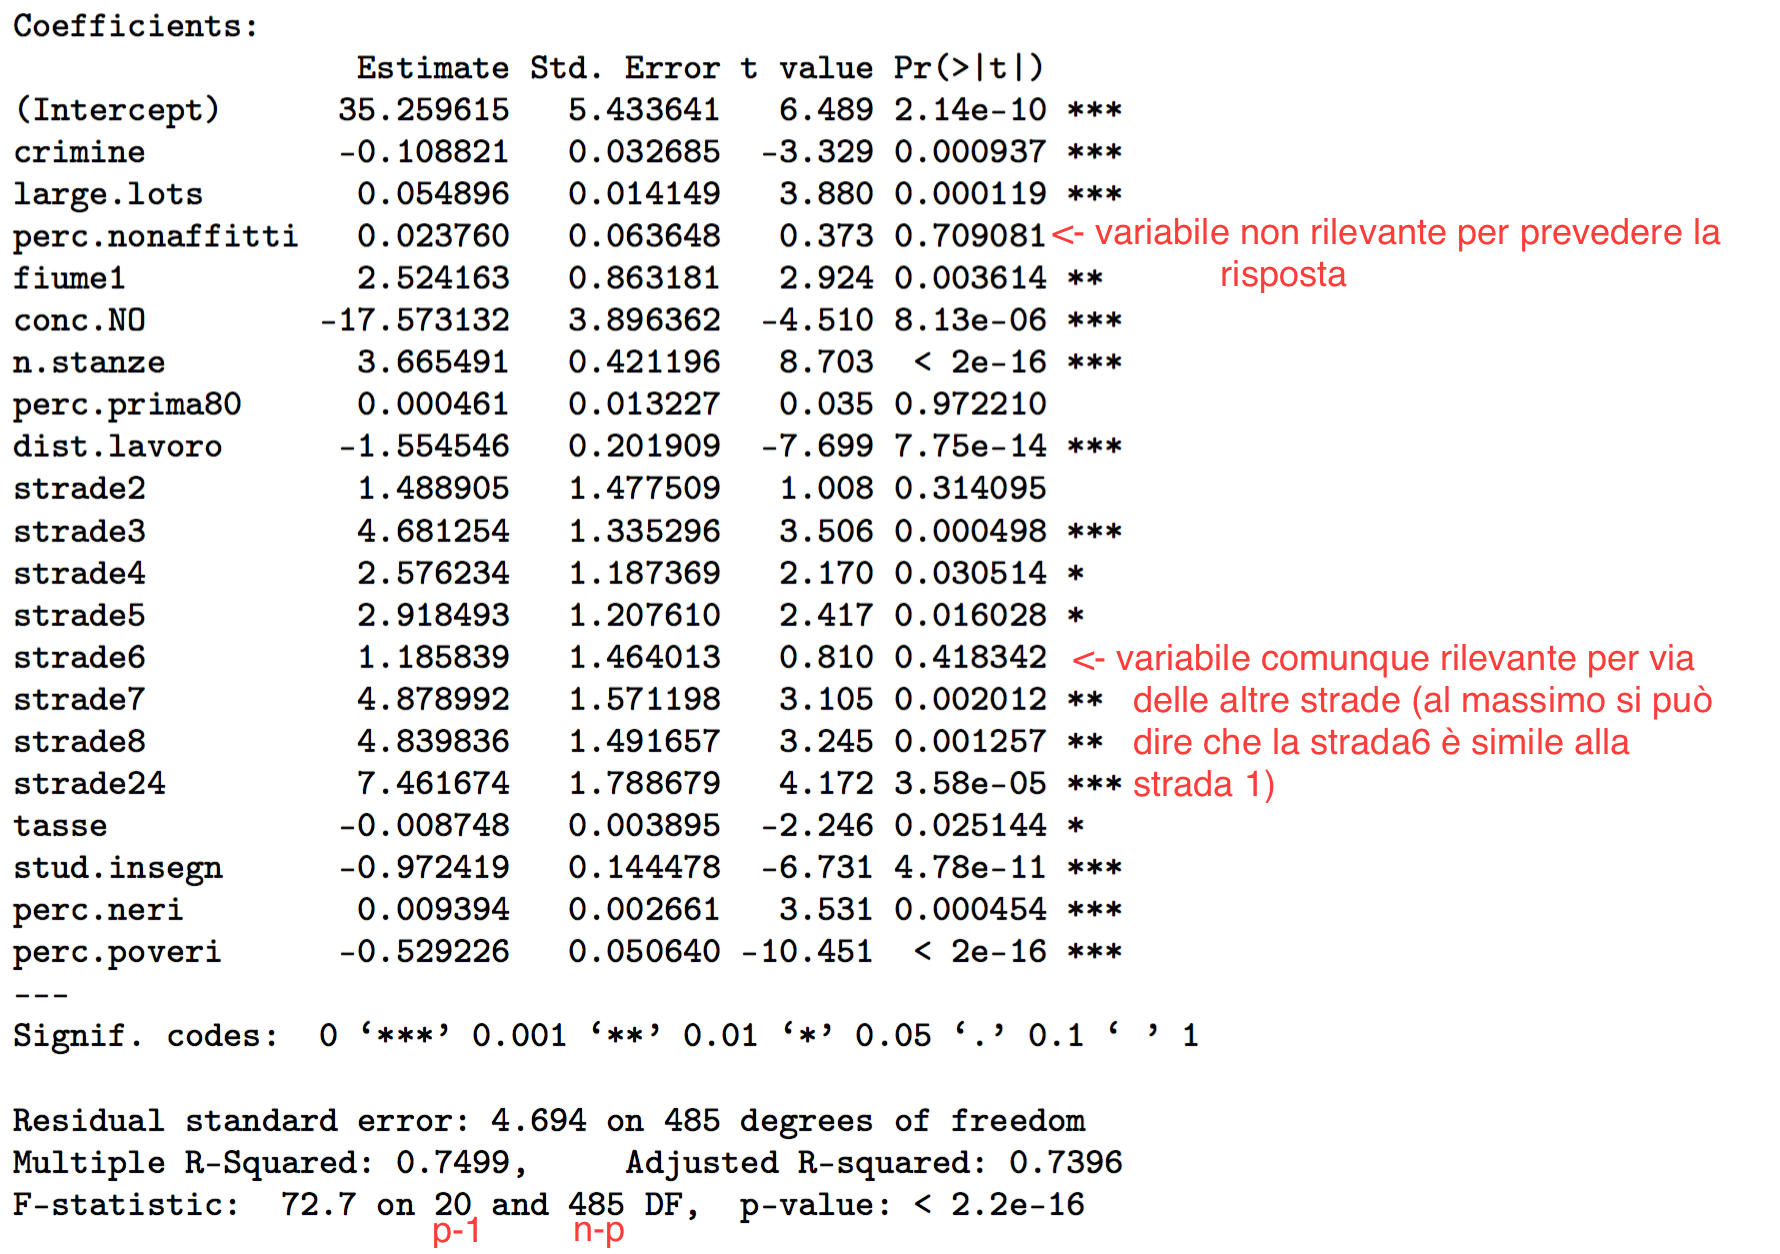
\includegraphics[width=.7\textwidth]{./notes/immagini/l10-fig1.png}
\end{figure}

\subparagraph{Dimostrazione}\label{dimostrazione-1}

Siano $ z_i $ e $ z_{i+p} $ dure caratteri di \textit{Z} a distanza \textit{p}. Siccome $ |\gamma|  \geq p$, i due caratteri possono essere appartenenti solamente o a \textit{X} o a \textit{Y} e mai ad entrambe le stringhe contemporaneamente. 
Pertanto dal momento che sia \textit{X} sia \textit{Y} hanno periodo \textit{p}, i due caratteri devono essere per forza uguali.

Da questo segue il lemma di periodicità che afferma che due periodi distinti \emph{p} e \emph{q} non possono coesistere troppo a lungo in
una stessa stringa senza che la stringa abbia anche periodo \emph{MCD(p,q)}.

\paragraph{Lemma - Lemma di periodicità}\label{lemma---lemma-di-periodicituxe0}

Sia \emph{X} una stringa di lunghezza \emph{n} con due periodi \emph{p}
e \emph{q} non entrambi nulli.

Se $n \geq p + q - MCD(p,q)$ allora la stringa \emph{X} ha anche periodo \emph{MCD(p,q)}.

\begin{figure}[htbp]
\centering
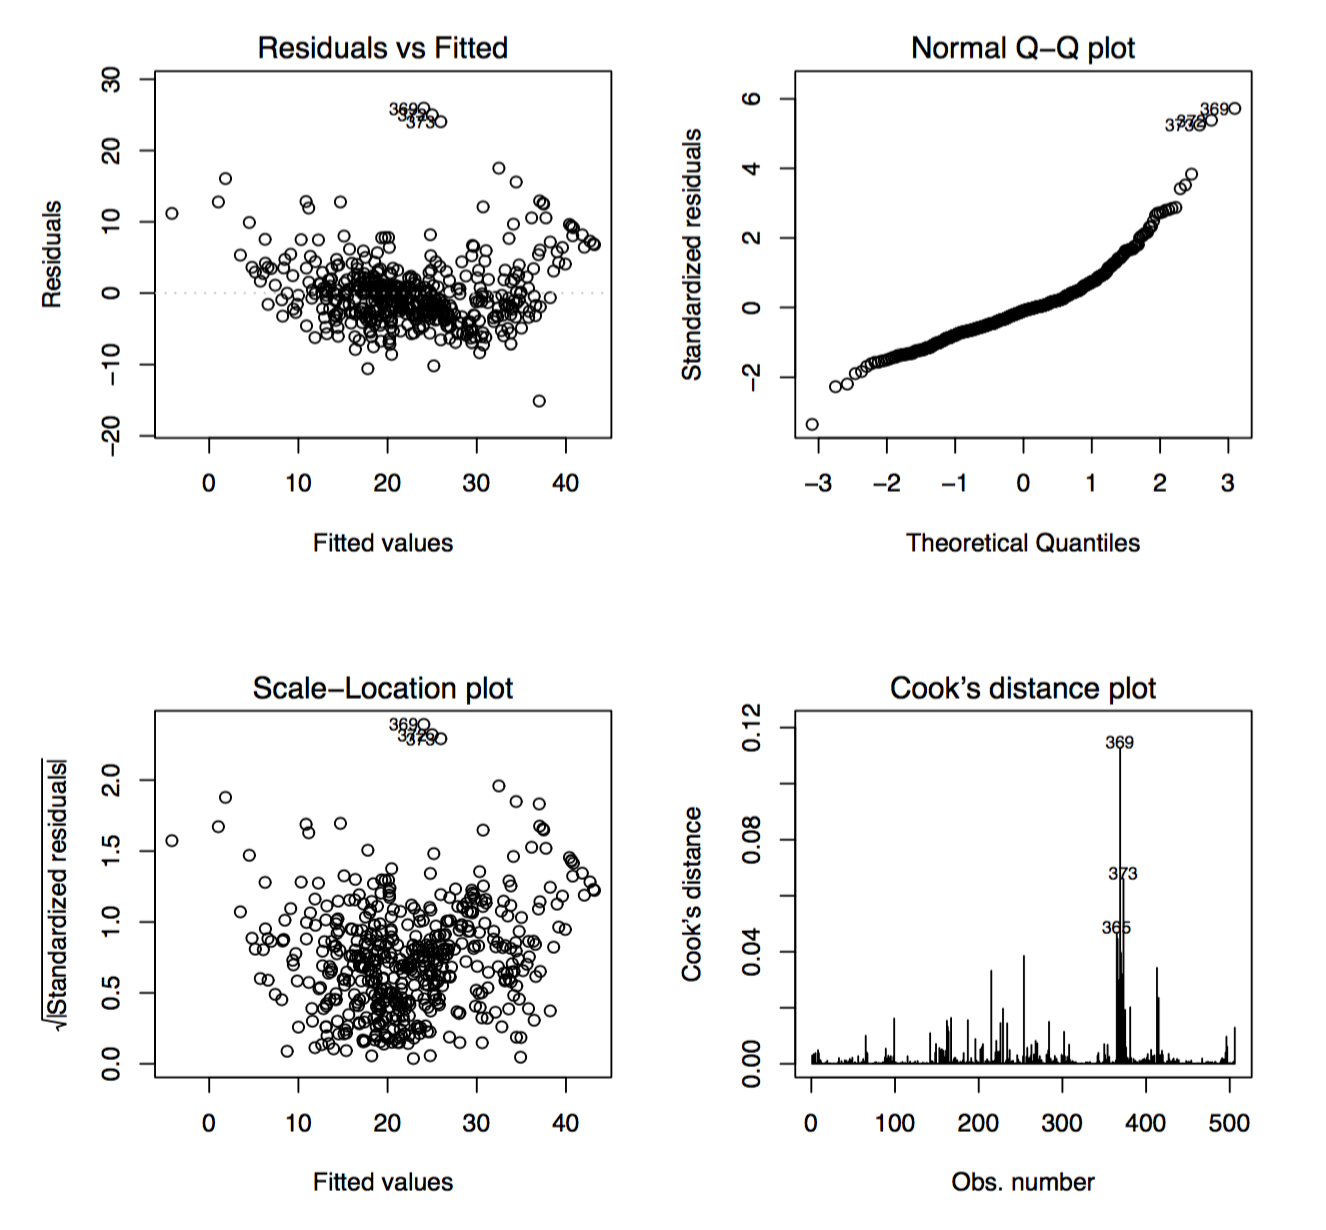
\includegraphics[width=.7\textwidth]{./notes/immagini/l10-fig2.png}
\caption{}
\end{figure}

\subparagraph{Dimostrazione}\label{dimostrazione-2}

Supponendo che $p \leq q$, la dimostrazione viene fatta per induzione su $p+q$.

$(p+q = 1)$ 

Se \emph{p=0} oppure \emph{p=q=0} allora \emph{MCD(p,q) = q} e dunque
\emph{X} ha periodo \emph{MCD(p,q)} perché ha periodo \emph{q}.

$(p+q > 1)$

Se \emph{p=0} o \emph{p=q} vale ancora il caso base.

Se $1 \leq p < q$, si ha che la stringa \emph{X} ha bordi $\alpha$ e $\beta$ di lunghezza \emph{n-p} e \emph{n-q}, questo per il primo lemma dimostrato.

\begin{figure}[htbp]
\centering
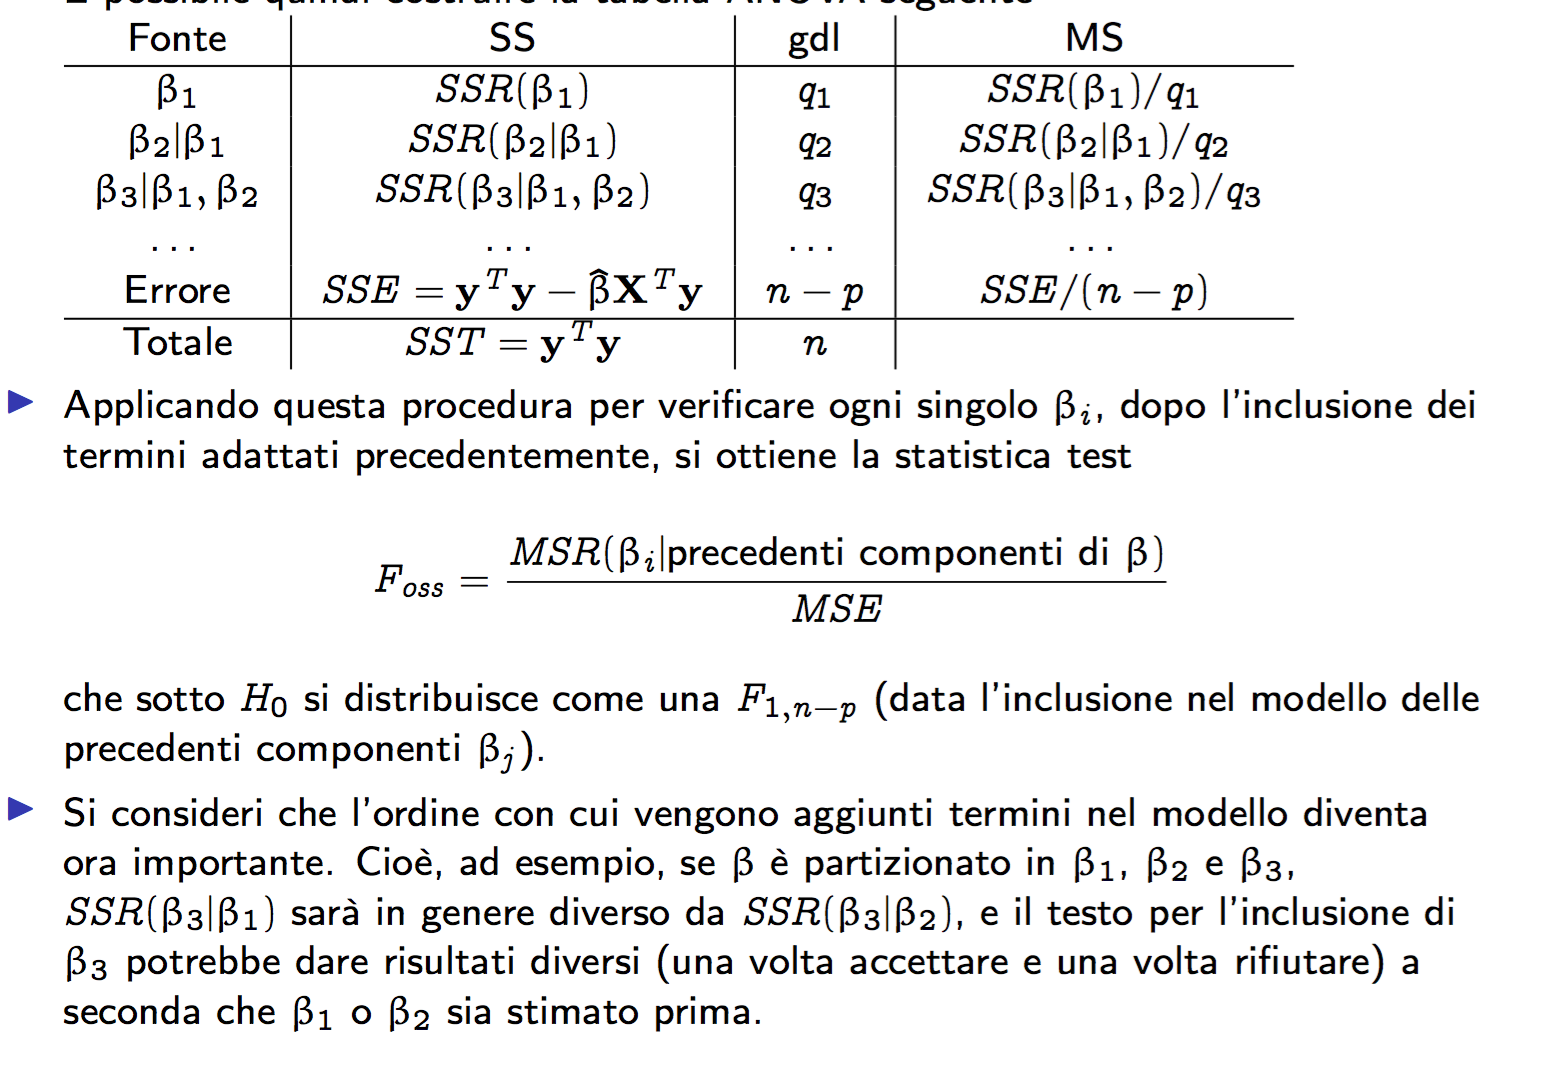
\includegraphics[width=.7\textwidth]{./notes/immagini/l10-fig3.png}
\caption{In verde la stringa $\alpha$ che si ripete con periodo
\emph{p}. In blu la stringa $\beta$ che si ripete con periodo
\emph{q}}
\end{figure}

La stringa $\beta$ essendo bordo di \emph{X} è anche bordo di $\alpha$ dal momento che $\alpha$ è un bordo di \emph{X}, pertanto $\alpha$ ha periodo $r = |\alpha| - |\beta| = q -p$.

Si ha che $p+r < p + q$, quindi è possibile applicare l'ipotesi induttiva, e che \emph{MCD(p,r) = MCD(p,q)}:

\begin{align*}
|\alpha| &\geq p+r-MCD(p,q)\\
 n - p &\geq q - MCD(p,q) 
\end{align*}

$ \alpha $ ha quindi come periodo sia \textit{r} (a causa di $ \beta $), sia \textit{p} (perché è una sottostringa di \textit{X}, la quale ha periodo \textit{p}) e per ipotesi induttiva ha anche periodo $MCD(p,r)$ che per come è definito \textit{r} è uguale a $MCD(p,q)$.

Considerando inoltre che:

\begin{align*}
	2|\alpha| &= (n-p) + (n-p) \\
					 &\geq q - MCD(p,q) + (n-p) \\
					 &\geq n
\end{align*}

perché $ p < q $ per ipotesi e $ MCD(p,q) \leq q - p $ per le proprietà del massimo comun divisore.

Questo implica che il prefisso $ \alpha $ di \textit{X} e il suffisso $ \alpha $ di \textit{X} coprono tutto \textit{X} e pertanto le due stringhe devono sovrapporsi\footnote{Non è possibile applicare il lemma della concatenazione perché non si sa di quanto queste stringhe si sovrappongono.} oppure $ X = \alpha\alpha $.

Presi quindi due caratteri $ x_i $ e $ x_j $ della stringa \textit{X}, tali che $ j - i = MCD(p,q) $ può succedere che i due caratteri appartengano alla stessa $ \alpha $ e quindi siano uguali, perché $ \alpha $ ha periodo $ r = MCD(p,q) $ oppure che $x_i \in \alpha_{(prefisso)} \text{ e } x_j \in \alpha_{(suffisso)} $.

\begin{figure}[htbp]
	\centering
	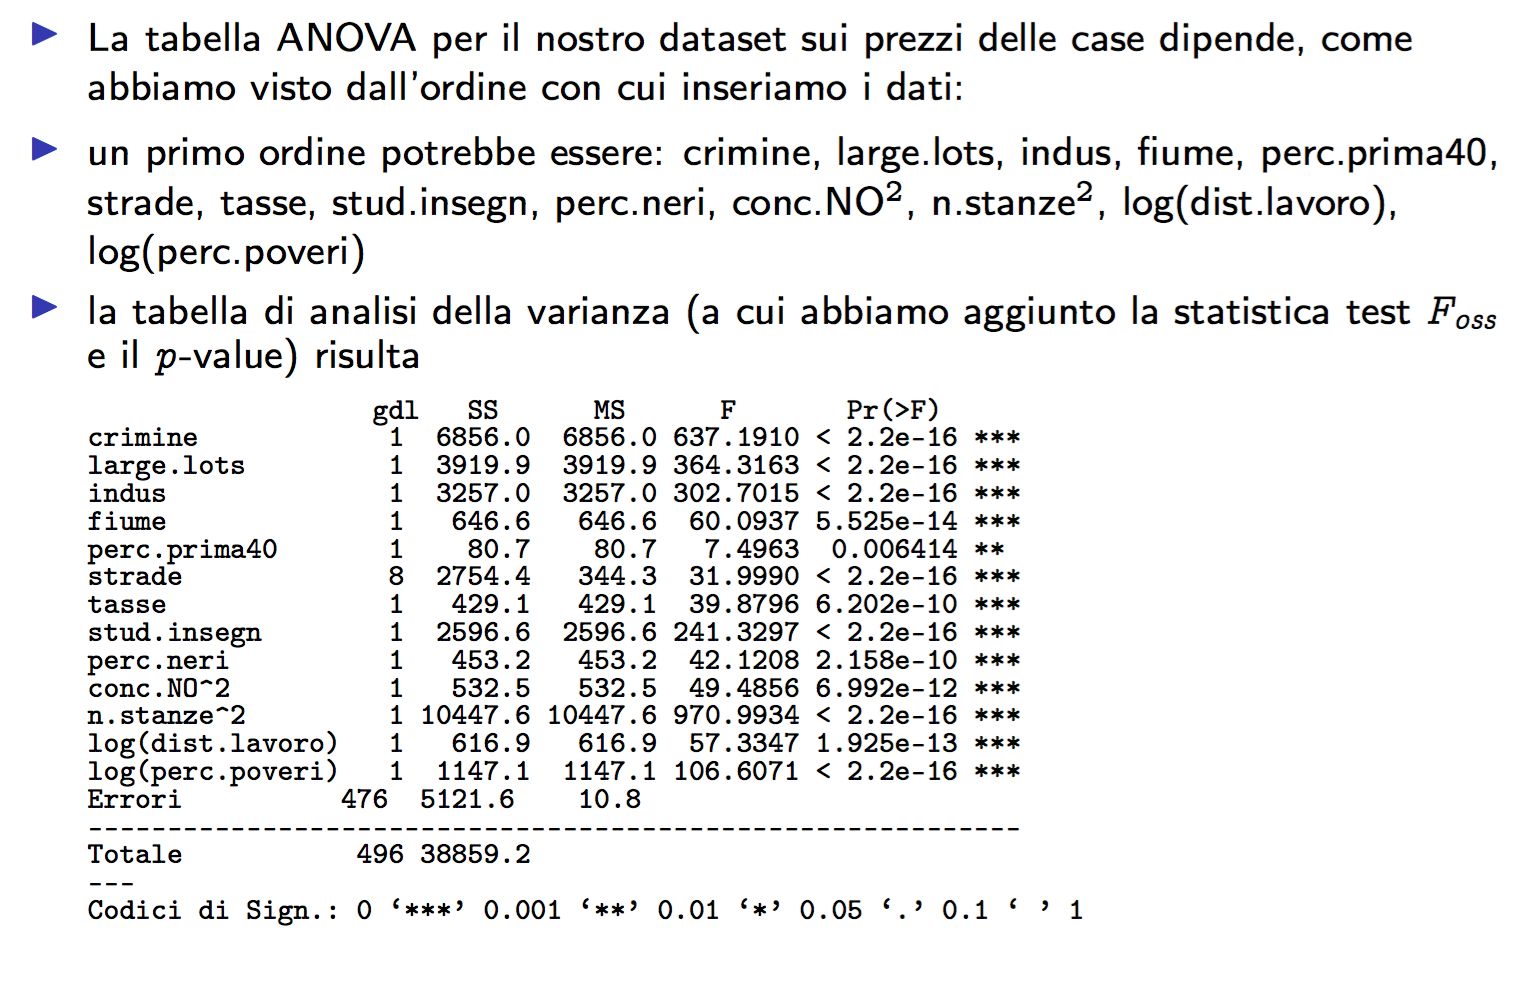
\includegraphics[width=.7\textwidth]{./notes/immagini/l10-fig4.png}
\end{figure}


In questo caso si ha che $ j > n - |\alpha| = p $ e quindi $ j - p \geq 1$. Si può quindi considerare il carattere $ x_{j-p} = x_j$ per via del periodo \textit{p} di $ X $ e che risulta appartenere a $ \alpha_{(prefisso)} $ perché $ p \geq MCD(p,q) $.

La distanza tra $ x_{j-p} \text{ e } x_i$ è $p - MCD(p,q)$, che per definizione è un multiplo di \textit{MCD(p,q)}, pertanto si ha che $ x_{j-p} \text{ e } x_i$ appartengono ad $ \alpha_{(prefisso)} $ che ha periodo \textit{MCD(p,q)}, pertanto $ x_{j-p} = x_i = x_j $ e di conseguenza \textit{X} ha periodo \textit{MCD(p,q)}.



\appendix
\chapter{Laboratorio}

\section{Un po' di cose su R}\label{un-po-di-cose-su-r}

\begin{itemize}
\item
  Tutti gli oggetti sono vettori
\item
  \texttt{ls()} per vedere le variabili disponibili
\item
  \texttt{x\ \textless{}-\ c(2,3,4,5)} crea un vettore con 1,2,3,4.
\item
  notazione \texttt{{[}1:20{]}} per un vettore con la successione da 1 a
  20
\item
  \texttt{xx\ \textless{}-\ seq(from=100,\ to=1)} crea sempre una
  sequenza di numeri, con parametro opzionale \texttt{by} per
  specificare lo step
\item
  \texttt{rep(2,5)} crea un vettore con 5 elementi uguali a 2
\item
  \texttt{a\ \textless{}-\ c(rep(2,3),4,5,rep(1,5))},
  \texttt{a\ =\ 2\ 2\ 2\ 4\ 5\ 1\ 1\ 1\ 1\ 1}
\item
  \texttt{2*x} esegue il prodotto scalare
\item
  \texttt{length(x)} per la lunghezza del vettore
\item
  \texttt{max(x)} e \texttt{min(x)}
\item
  \texttt{sum(x)} che ritorna un vettore di un solo elemento con la
  somma
\item
  \texttt{mean(x)}, \texttt{var(x)}, \texttt{range(x)}
\item
  \texttt{x{[}7{]}} per estrarre il settimo elemento di \texttt{x},
  l'indice credo parta da 1
\item
  \texttt{x{[}-4{]}} ritorna un vettore senza il quarto elemento
\item
  \texttt{x\ \textless{}-\ matrix(c(2,3,5,7,11,13),nrow\ =\ 3)} crea una
  matrice con gli elementi specificati e 3 righe. Alternativamente è
  possibile specificare anche il numero di colonne.
\item
  \texttt{x2\ \textless{}-\ scan("nome\ file",\ sep="")} con
  \texttt{sep} opzionale, per caricare il contenuto di un file in un
  vettore, per caricare una matrice
  \texttt{x2\ \textless{}-\ matrix(scan(...),\ ncol\ =\ 3,\ byrow=TRUE}.
\item
  \texttt{str(x)} specifica la struttura dell'oggetto
\item
  \texttt{dim(x)} ritorna la dimensione di una matrice, se invocato con
  un vettore ritorna \texttt{NULL}.
\item
  \texttt{x{[}18,{]}} per ottenere la 18-esima riga di una matrice
\item
  \textbf{Dataframe}: matrice le cui colonne possono avere formati
  diversi
\item
  \texttt{ciliegi\ \textless{}-\ read.table("nome\ file")}.
\item
  \texttt{names(ciliegi)} è il vettore con i nomi delle colonne del
  dataframe
\item
  \texttt{names(ciliegi)\ \textless{}-\ c("diametro",\ "altezza",\ "volume")}
  permette di impostare il nome delle colonne, può anche essere
  specificato come parametro opzionale \texttt{col.names} della
  funzione \texttt{read.table}.
\item
  \texttt{summary(ciliegi)} fornisce degli indicatori per ciascuna
  colonna
\item
  \textbf{Mediana}: elemento centrale di una distribuzione ordinata in
  senso crescente, \textbf{primo e terzo quartile}: generalizzazione
  della mediana, rispettivamente l'elemento che sta al 25 e 75 per cento
  della distribuzione. La differenza tra i due quartili da l'idea di
  quanto è variabile la distribuzione.
\item
  I dataframe possono essere acceduti anche con il nome della colonna
  \texttt{ciliegi\$volume}.
\item
  \textbf{attach di un file}: aggiungere al workspace un oggetto, ovvero
  \texttt{attach(ciliegi)} permette di accedere al nome della colonna
  direttamente utilizzando \texttt{volume}. Come complementare c'è il
  comando \texttt{detach}.
\item
  \texttt{hist(diametro)} crea l'istogramma per il diametro
\item
  \texttt{help(hist)} per avere l'help di una funzione
\item
  l'istrogramma che viene generato di default può contenere dei buchi,
  conviene quindi adattare il numero di colonne utilizzando il parametro
  \texttt{breaks}
\item
  \texttt{boxplot(diametro)} fornisce il box plot di un valore, è un
  grafico che rappresenta la mediana, i quartili e il 5 e 95\%. Risulta
  più espressivo dell'istogramma. L'ampiezza della scatola rappresenta
  la variabilità dei dati.
\item
  \texttt{ciliegi{[}altezza\textgreater{}80,{]}} prende tutti i ciliegi
  con altezza maggiore di 80.
\item
  \texttt{library(MASS)} permette di caricare la libreria MASS
\item
  \texttt{search()} permette di visualizzare la lista degli ottetti in
  cui R va a cercare quando deve eseguire un comando
\item
  Gli attributi qualitativi vengono trattati come tipo Factor
\item
  \texttt{table(painters\$School)} crea la tabella con le frequenze
  delle varie qualità
\item
  \texttt{barplot(..)} fa il plot delle barre per una variabile discreta
\item
  \texttt{pie(...)} fa il grafico a torta, anche se è sconsigliabile
  utilizzare un grafico a torta perché per l'occhio umano fa fatica a
  vedere la differenza tra gli angoli.
\item
  come scale colori si possono utilizzare \texttt{heat.colors(k)},
  \texttt{rainbow(k)}, \ldots{}
\item
  \texttt{plot(x,y)} disegna un diagramma di dispersione, il parametro
  \texttt{pch} specifica il tipo di carattere, \texttt{pch=16}
  rappresenta i pallini pieni, \texttt{col} specifica il colore da
  utilizzare, possono indicare \texttt{col=painter\$School} per far
  variare il colore in base al valore dell'attributo quantitativo
\end{itemize}

%% !TEX encoding = UTF-8
% !TEX TS-program = pdflatex
% !TEX root = computabilità e algoritmi.tex
% !TEX spellcheck = it-IT
\section{Composizione generalizzata}\label{composizione-generalizzata}

$$f: \mathbb{N}^k \rightarrow \mathbb{N},\: g_1,\ldots g_n : \mathbb{N}^k \rightarrow \mathbb{N}$$

La loro composizione $h: \mathbb{N}^k \rightarrow \mathbb{N}$ è data da: 

$$
h(\vec{x}) = f(g_1(\vec{x}), \ldots, g_n(\vec{x}))
$$

La funzione $h(\vec{x})\downarrow$ (è definita) se tutte le
$g_i \downarrow y_i, f(y_1,\ldots,y_n) \downarrow$.

L'approccio utilizzato nella valutazione delle funzioni è quello
\textbf{eager}, ovvero vengono valutati prima tutti i parametri.

Ad esempio: $\underline{0} : \mathbb{N} \rightarrow \mathbb{N},\: \underline{0}(x) = 0$ e $d(x) = \uparrow,\: \underline{0}(d(1))$ è
$\uparrow$ perché prima è necessario valutare i parametri.

\subsection{Calcolabilità della funzione
composta}\label{calcolabilituxe0-della-funzione-composta}

Se $f: \mathbb{N}^n \rightarrow \mathbb{N}, g_1\ldots g_n : \mathbb{N}^k \rightarrow \mathbb{N} \in \mathcal{C}$, allora anche $h: \mathbb{N}^k \rightarrow \mathbb{N}$ è calcolabile in $\mathcal{C}$.

\subsubsection{Dimostrazione}\label{dimostrazione}

Siano $F,G_1, \ldots{}, G_n$ programmi URM in forma normale per
le relative funzioni.

L'input della funzione \emph{h} avrà nei primi \emph{k} registri i
valori di input, è necessario quindi andare a copiarli in una locazione
di memoria che non viene usata dai vari programmi, ovvero dalla
locazione \emph{m+1}, con $m = max\{\rho(F), \rho(G_1), \ldots \rho(G_N), k,n\}$.

I risultati parziali dei programmi vengono poi memorizzati a partire
dalla locazione \emph{m + k +1} per poi essere utilizzati da \emph{F}

Il programma risultante è:

\begin{lstlisting}[language=URM]
T([1 ... k],[m+1 ... m+k])
G1[m+1 ... m+k -> m+k+1]
...
Gn[m+1 ... m+k -> m+k+n]
F[m+k+1 ... m+k+n -> 1]
\end{lstlisting}

\subsubsection{Esempio - Somma di due numeri}\label{esempio}

A partire dalla funzione $sum(x_1, x_2) = x_1+x_2$ è possibile andare a ottenere la funzione

$$f(x_1, x_2, x_3) = x_1 + x_2 +x_3$$

componendo la funzione \textit{sum} con se stessa:

$$f(x_1, x_2, x_3) = sum(sum(x_1,x_2),x_3)$$

Tuttavia, strettamente parlando, le $g_i$ non hanno la stessa
arietà, pertanto sono necessari dei piccoli aggiustamenti:

$$f(x_1, x_2, x_3) = sum(sum(U_1^{3}(\vec{x}),U_2^3(\vec{x}))), U_3^3(\vec{x}))$$

\section{Ricorsione Primitiva}\label{ricorsione-primitiva}

\begin{align*}
	fact(0) &= 1 \\
	fact(n+1) &= (n+1)fact(n)
\end{align*}

\begin{align*}
	fib(0) &= 1 \\
	fib(1) &= 1 \\
	fib(n+2) &= fib(n+1) + fib(n)
\end{align*}

Date $f: \mathbb{N}^k \rightarrow \mathbb{N}$ e $g:\mathbb{N}^{k+2} \rightarrow \mathbb{N}$, la funzione per ricorsione primitiva $h: \mathbb{N}^{k+1} \rightarrow \mathbb{N}$ è definita come

\begin{align*}
	h(\vec{x}, 0) &= f(x) \\
	h(\vec{x}, y+1) &= g(\vec{x}, y, h(\vec{x},y))
\end{align*}

Così facendo viene definita \emph{h} utilizzando \emph{h} e
concettualmente è corretto, tuttavia è necessario dimostrare formalmente
l'esistenza e l'unicità di \emph{h}.

Questo lo si fa considerando l'operatore $\Phi$:

\begin{align*}
	\Phi : (\mathbb{N}^k \rightarrow \mathbb{N}) &\rightarrow (\mathbb{N}^k \rightarrow \mathbb{N}) \\
	\Phi(h)(\vec{x}, 0) &= f(\vec{x}) \\
	\Phi(h)(\vec{x}, y+1) &= g(\vec{x}, y, h(\vec{x},y))
\end{align*}

tale che $\Phi(h) = h$, ovvero tale che viene raggiunto un punto
fisso. Ciò sarebbe da dimostrare, ma questo va oltre l'obiettivo del corso, quindi viene dato per buono.

In altre parole, se \emph{h} rispetta lo schema precedentemente definito, allora esiste ed è unica.

Assumendo quindi che la ricorsione primitiva di una funzione calcolabili
è calcolabile, è possibile definire varie operazioni senza scrivere
esplicitamente il programma per calcolarle:

Ad esempio la funzione somma può essere definita in modo ricorsivo:

$$
	x+y = h(x,y) =\begin{cases}
	x+0 = x &\Rightarrow f(x) = x \\
	x+(y+1) = (x+y) + 1 &\Rightarrow g(x,y,z) = succ(z)
	\end{cases}
$$

In modo simile possono essere anche definiti il prodotto e l'esponenziale:

$$
x \cdot y = h(x,y) =\begin{cases}
x \cdot 0 = 0 &\Rightarrow f(x) = 0 \\
x \cdot (y+1) = (x \cdot y) + x &\Rightarrow g(x,y,z) = z+x
\end{cases}
$$

$$
x^y = h(x,y) =\begin{cases}
x^0 = 1 &\Rightarrow f(x) = 1 \\
x^{(y+1)} = (x^y) \cdot x &\Rightarrow g(x,y,z) = z \cdot x
\end{cases}
$$

\subsection{Calcolabilità della Ricorsione Primitiva}\label{calcolabilituxe0-della-ricorsione-primitiva}

Siano $f:\mathbb{N}^k \rightarrow \mathbb{N}$ e $g:\mathbb{N}^{k+2} \rightarrow \mathbb{N} \in \mathcal{C}$ allora anche \emph{h} definita per
ricorsione primitiva è in $\mathcal{C}$. Ovvero quello che è stato assunto precedentemente.

\subsubsection{Dimostrazione}\label{dimostrazione-1}

Siano \emph{F} e \emph{G} i programmi che calcolano \emph{f} e \emph{g}.

Il programma che calcola \emph{h} verrà invocato con il vettore \emph{x}
nelle prime \emph{k} locazioni e con \emph{y} nella locazione
\emph{k+1}.

Come prima cosa è necessario trasferire i dati di input in una zona di
memoria non utilizzata dai programmi \emph{F} e \emph{G}, ovvero
\emph{m+1}, dove $m = max\{\rho(F), \rho(G), k+2\}$.

Dopodiché è necessario effettuare un'interazione su un contatore
\emph{i} che parte da 0, fino a quando non viene raggiunto \emph{y}.

\begin{verbatim}
h(vec(x), 0) = f(vec(x)) -- i=0 -- i==y? NO
h(vec(x), 1) = g(vec(x), 0, h(vec(x),0)) -- i=1 -- i==y? NO
...
h(vec(x), i+1) = g(vec(x), i, h(vec(x),i)) -- i=n -- i==y? SI -> fine
\end{verbatim}

ovvero il programma per \emph{h} sarà:

\begin{lstlisting}[language=URM]
T([1..k], [m+1 ... m+k]) // copia x
T(k+1, m+k+3) //copia y
F[m+1 ... m+k -> m+k+2]
J(m+k+3, m+k+1, END) #LOOP
G[m+1 ... m+k+2 -> m+k+2] // h(vec(x),i+1)
S(m+k+1) //i++
J(1,1,LOOP)
T(m+k+2,1) #END
\end{lstlisting}

Se \emph{f} e \emph{g} sono funzioni parziali quanto dimostrato richiede
maggiori precisazioni, ma a noi basta sapere che se durante il calcolo
troviamo qualche funzione non definita, anche \emph{h} non è definita.

\subsection{Funzioni totali definite ricorsivamente}\label{osservazione-senza-titolo}

Le funzioni definite a parte da funzioni totali mediante composizione o
ricorsione sono anche loro totali.

La dimostrazione per le funzioni mediante composizione è vera per
definizione, l'altra è lasciata per esercizio (si fa per induzione).

\todo[inline]{todo}

\subsection{Esercizio - Libreria di funzioni calcolabili}\label{esercizio---libreria-di-funzioni-calcolabili}

\begin{itemize}
\item
  somma \emph{x+y}
\item
  prodotto $x \cdot y$
\item
  esponenziale $x^y$
\item
  fattoriale \emph{fact(x)}
\end{itemize}

Sguardo d'insieme: vogliamo trovare un programma URM in grado di
simulare un altro programma URM, le operazioni numeriche sono
interessanti perché il programma in input verrà rappresentato come un
numero.

\subsubsection{Predecessore}\label{predecessore}

$$ \text{pred}(x) = \begin{cases}x \dotminus 1 = 0, \:& \text{ se } x=0\\
x-1, \:& \text{ se } x > 0\end{cases}$$

Può essere calcolata ricorsivamente con

\begin{align*}
	0 \dotminus 1 &= 0 \\
	(y+1) \dotminus 1 &= y
\end{align*}

\subsubsection{Sottrazione tra numeri naturali}\label{sottrazione-tra-numeri-naturali}

$$x \dotminus y =\begin{cases}
0,\:& \text{se } x \leq y\\
x-y, \:& \text{altrimenti}
\end{cases}$$

Può essere calcolata ricorsivamente con:

\begin{align*}
x \dotminus 0 &= x \\
x\dotminus (y+1) &= (x \dotminus y) \dotminus 1
\end{align*}

\subsubsection{Segno}\label{segno}

$$sg(x) =\begin{cases}
0,\:& \text{se } x = 0\\
1, \:& \text{altrimenti}
\end{cases}$$

Può essere calcolata ricorsivamente con:

\begin{align*}
sg(0) &= 0 \\
sg(y+1) &= 1
\end{align*}

In modo simile può essere definito anche $\overline{sg}$.

\subsubsection{Valore assoluto della differenza}\label{valore-assoluto-della-differenza}

$$|x - y|=\begin{cases}
x-y,\:& \text{se } x \leq y\\
y-x, \:& \text{altrimenti}
\end{cases}$$

Può essere calcolata in modo composizionale con:

$$|x - y| = (x \dotminus y) + (y \dotminus x)$$


\subsubsection{Minimo}\label{minimo}

$$ \min (x,y) =\begin{cases}
x,\:& \text{se } x \leq y\\
y, \:& \text{altrimenti}
\end{cases}$$

Può essere calcolata con:

$$\min(x,y) = x \dotminus (x \dotminus y)$$

Questo perché se \emph{x} è il minimo, $x\dotminus y$ è 0.

\subsubsection{Resto della divisione intera}\label{resto-della-divisione-intera}

$$\text{rm}(x,y) =\begin{cases}
y \mod x,\:& \text{se } x \neq y\\
y, \:& \text{altrimenti}
\end{cases}$$


Può essere calcolato ricorsivamente come:

\begin{align*}
\text{rm}(x,0) &= 0 \\
\text{rm}(x, y+1) &= \begin{cases}\text{rm}(x+y) +1, \:& \text{ se rm}(x+y) +1 \neq x\\
0, \:& \text{ altrimenti} \end{cases}
\end{align*}

L'\emph{if} può essere espresso in modo algebrico utilizzando la
funzione \emph{sg}, ottenendo:

$$\text{rm}(x, y+1) = (sg(x \dotminus \text{rm}(x,y) \dotminus 1))(\text{rm}(x,y)+1)$$

\subsubsection{Esercizio - Divisione intera}\label{esercizio---divisione-intera}

$$\text{qt}(x,y) =\begin{cases}
\floor[\Big]{\frac{y}{x}},\:& \text{se } x \neq y\\
y, \:& \text{altrimenti}
\end{cases}$$

\todo[inline]{todo}

\subsubsection{Esercizio - Definizione per casi}\label{esercizio---definzione-per-casi}

$f_1 \ldots f_n : \mathbb{N}^k \rightarrow \mathbb{N}$ totali e calcolabili e
$Q_1, \ldots, Q_n \subseteq \mathbb{N}^k$ decidibili e tali che per ogni $\vec{x}$ solo un predicato è vero.

Definire $f(x) = f_1(x) \text{ se } Q_1(x) \ldots f_n(x) \text{ se } Q_n(x)$

\todo[inline]{todo}

% !TEX encoding = UTF-8
% !TEX TS-program = pdflatex
% !TEX root = data mining.tex
% !TEX spellcheck = it-IT
\chapter{Formulario}
%(a - b)(a -b) = aa -ab +bb -ab
\section{Formule generiche}

\begin{align*}
\var(X) &= \frac{\sum\limits_{i=1}^n (x_i - \bar{x})^2}{n}
= \frac{ \sum\limits_{i=1}^n ( x_i^2 + \bar{x}^2   - 2 x_i \bar{x}) }{n}
= \frac{ \sum\limits_{i=1}^n x_i^2 + n\bar{x}^2 -2\bar{x} \sum\limits_{i=1}^n x_i }{ n} \\
&= \frac{\sum_{i=1}^{n} x_i^2}{n} - \bar{x}^2
\end{align*}

\begin{align*}
\cov(X,Y) &= \frac{\sum\limits_{i=1}^n (x_i - \bar{x})(y_i - \bar{y})}{n}
= \frac{ \sum\limits_{i=1}^n (x_iy_i - x_i\bar{y} -\bar{x}y_i + \bar{x}\bar{y})}{n}
= \frac{ \sum\limits_{i=1}^n x_iy_i -\bar{y}\sum\limits_{i=1}^n x_i -\bar{x}\sum\limits_{i=1}^ny_i + n\bar{x}\bar{y}}{n} \\
&= \frac{\sum\limits_{i=1}^{n} (x_iy_i)}{n} - \bar{x}\bar{y}
\end{align*}

\subsection{Coefficiente di correlazione di Pearson}

$$
\rho_{YX_1:X_2} = \frac{\cov(Z_Y, Z_{X_1})}{\sqrt{\var(Z_Y)\var(Z_{X_1})}}
$$

$$
-1 \leq \rho_{YX_1:X_2} \leq 1
$$

Se $\rho_{YX_1:X_2} = 0$ le variabili $ Y $ e $ X_1 $ non sono correlate, se invece vale 1 o $ -1 $ sono correlate (direttamente o indirettamente).

\subsection{Scomposizione della varianza}

$$
\underbrace{\sum\limits_{i=1}^n (y_i - \bar{y})^2}_{\text{SST: devianza}} = 
\underbrace{\sum\limits_{i=1}^n (y_i - \hat{y}_i)^2}_{\text{SSE: devianza residua}}  +
\underbrace{\sum\limits_{i=1}^n (\hat{y}_i - \bar{y})^2}_{\text{SSR: devianza spiegata dal modello}}
$$

$$
\underbrace{\vec{y}^T\vec{y}}_{\textbf{SST}: \text{somma dei quardati totale}} = 
\underbrace{(\vec{y} - \vec{\bar{y}})^T (\vec{y} - \vec{\bar{y}})}_{\textbf{SSE}: \text{somma dei quadrati degli errori}} +
\underbrace{\vec{\hat{\beta}} \textbf{X}^T\vec{y}}_{\textbf{SSR}: \text{somma dei quadrati della regressione}}
$$

\section{Modello lineare}

\begin{align*}
S^2(\beta_0, \beta_1) = \sum\limits_{i=1}^n (y_i - \beta_0 - \beta_1 x_i)^2
\end{align*}

\begin{align*}
\hat{\beta}_1 &= \frac{\cov(X,Y)}{\var(X)} 
= \frac{\sum\limits_{i=1}^n (x_i - \hat{x})(y_i - \bar{y})}{\sum\limits_{i=1}^n (x_i - \bar{x})^2} 
= \frac{\sum\limits_{i=1}^n (x_i - \bar{x})y_i}{\sum\limits_{i=1}^n (x_i - \bar{x})^2}  \\
%
\hat{\beta}_0 &= \bar{y} - \hat{\beta}_1 \bar{x}
\end{align*}

\subsection{Residui}

$$
r_i = y_i - \hat{\beta}_0 - \hat{\beta}_1 x_i
$$

\begin{align*}
\var(R) &= \frac{1}{n}\sum\limits_{i=1}^n r_{i}^2
= \var(Y) - \frac{\cov^2(X,Y)}{\var(X)}
\end{align*}

\subsection{Coefficiente di determinazione}

$$
R^2 = 1 - \frac{\var(R)}{\var(Y)}
$$


\subsection{Stima della varianza della distribuzione}

La varianza degli errori può essere approssimata con la varianza dei residui, scalata per un opportuno fattore, che potrebbero essere i gradi di libertà della distribuzione dei residui.
Nel caso della regressione lineare a due parametri si ha che i gradi di libertà sono $ n - p  = n-2 $

\begin{align*} 
\hat{s}^2 &= \frac{1}{n-2}\sum\limits_{i=1}^n (r_{i} - 0)^2\\
				 &= \frac{1}{n-2}\sum\limits_{i=1}^n (y_i - \hat{\beta}_0 - \hat{\beta}_1x_i)^2 \\
				 &= \frac{SSE}{n-p}
\end{align*}

\begin{align*}
	\var(\hat{\beta}_0) &= s^2 \bigg( \frac{1}{n} + \frac{\bar{x}^2}{\sum_{i=1}^{n} (x_i - \bar{x})^2}\bigg) = s^2 \bigg(\frac{\sum_{i=1}^{n}x_i^2}{n\sum_{i=1}^{n} (x_i - \bar{x})^2}\bigg) \\
	\var(\hat{\beta}_1) &= s^2 \bigg( \frac{1}{\sum_{i=1}^{n} (x_i - \bar{x})^2} \bigg)
\end{align*}

Varianza della stima, ha gli stessi gradi di libertà della varianza dei residui $n-p$:

$$
\widehat{\var(\hat{y}_0)} = s^2 \Bigg( 1 + \frac{1}{n} + \frac{(x_0 - \bar{x})^2}{\sum_{i=1}^{n} (x_i - \bar{x})^2} \Bigg)
$$

\subsection{Verifica delle ipotesi}
$ t_{oss} $ per $ \hat{\beta}_1 $
\begin{align*}
t_{oss} = \frac{(\hat{\beta}_1 - 0)}{\sqrt{\frac{s^2}{\sum_{i=1}^{n} (x_i - \bar{x})^2}}} \\
\Bigg[ \hat{\beta}_1 \pm t_{n-2, 1-\alpha/2}  \sqrt{\frac{s^2}{\sum_{i=i}^{n} (x_i - \bar{x})^2}}\Bigg]
\end{align*}

$ t_{oss} $ per $ \hat{\beta}_0 $
\begin{align*}
t_{oss}  = (\hat{\beta}_0 - \beta') \Bigg/ s \sqrt{\frac{\sum_{i=1}^{n} x_{i}^2}{n \sum_{i=1}^{n} (x_i - \bar{x})^2}} \\
\Bigg[ \hat{\beta}_0 \pm t_{n-2, 1-\alpha/2} \cdot s \cdot \: \sqrt{\frac{\sum_{i=1}^{n} x_{i}^2}{n \sum_{i=1}^{n} (x_i - \bar{x})^2}} \Bigg]
\end{align*}
\textbf{livello di significatività osservato} o \textbf{p-value}: indicatore uguale alla probabilità di osservare, supponendo vera $ H_0 $, un valore di $ t_{oss} $ uguale o ``più lontano'' da $ H_0 $ di quanto effettivamente è osservato, ovvero costituisce una misura di quanto l'ipotesi nulla è plausibile sulla base dei dati osservati.

$$
p-value = 2 \times P(t \text{con } n-p \text{ gradi} \geq t_{oss} )
$$

Per valutare l'andamento globale del modello è possibile utilizzare $ F_{oss} $ che si comporta in modo simile a $ t_{oss} $ con la differenza che la distribuzione di riferimento è la $ F $ di Snedecor con $ p-1 $ gradi di libertà al numeratore e $ n-p $ gradi di libertà al denominatore.

\begin{align*}
F_{oss} = \Bigg( \frac{R^2}{ 1 - R^2}\Bigg) \Bigg( \frac{n -k}{k-1} \Bigg) \\
k = \text{numero di parametri del modello}
\end{align*}



\subsubsection{Regola di accettazione/rifiuto}

\begin{enumerate}
	\item Fisso un intervallo di confidenza $ 1-\alpha $
	\item Calcolo, utilizzando le tavole $ t_{n-p, 1-\alpha/2} $
	\item Calcolo il $ t_{oss} $ opportuno (per $ \hat{\beta}_0 $ o$ \hat{\beta}_1 $)
	\item Controllo se $ | \: t_{oss}\: \leq t_{n-p, 1-\alpha/2}  $, se è vero accetto $ H_0 $, altrimenti la rifiuto.
\end{enumerate}



\section{Modello lineare con più variabili}

$$
Y = \beta_0 + \beta_1 X_1+\beta_2X_2 + \epsilon
$$

Minimi quadrati:

$$
s^2(\beta_0, \beta_1, \beta_2) = \sum\limits_{i=1}^n(y_i - \beta_0 + \beta_1 x_{1,i}+\beta_2 x_{2,i} )
$$

$$
\begin{cases}
\hat{\beta}_1 &= \frac{cov(X_1,Y)sqm(X_2) - cov(X_2, Y)cov(X_1,X_2)}{sqm(X_1)sqm(X_2)- cov^2(X_1,X_2)} \\
\hat{\beta}_2 &= \frac{cov(X_2,Y)sqm(X_1) - cov(X_1, Y)cov(X_1,X_2)}{sqm(X_1)sqm(X_2)- cov^2(X_1,X_2)}  \\
\hat{\beta}_0 &= \bar{y} - \hat{\beta}_1\bar{x}_1 - \hat{\beta}_2\bar{x}_2
\end{cases}
$$
% !TEX encoding = UTF-8
% !TEX TS-program = pdflatex
% !TEX root = data mining.tex
% !TEX spellcheck = it-IT
\chapter{Soluzioni Parziali}

\section{Aprile 2015}

\subsection{Esercizio 5}

\subsubsection{Domanda a}


\subsubsection{Domanda b}

Bisogna completare i dati dell'output.

I gradi di libertà per la $ F_{oss} $ sono 2 e 19, rispettivamente $ p-1 $ e $ n-p $ con \textit{p} numero di parametri. I gradi di libertà degli errori sono sempre $ n-p = 19 $.

Per calcolare $ RSE $ serve $ s^2 $ che è la stima della varianza degli errori (e dei residui).

$$
RSE = \sqrt{\frac{SSE}{n-p}} = \sqrt{\frac{\sum\limits_{i=1}^n (y_i - \hat{y}_i)^2}{n-p}} = \sqrt{s^2} 
$$

Sappiamo che:

$$
\widehat{\var(\vec{\hat{\beta}})} = (\textbf{X}^T\textbf{X})^{-1}s^2
$$

e che $ \sqrt{\var (\hat{\beta}_0)} = 126,758$ e $(\textbf{X}^T\textbf{X})_{11}^{-1} = 0,6363  $ da cui segue $ s^2 = \frac{126,758^2}{0,6363} =  25.251,596$, pertanto $ RSE = \sqrt{s^2} = 158,..$.

%----------------------------------------------------------------------------------------
% BIBLIOGRAPHY
%----------------------------------------------------------------------------------------
%\bibliographystyle{unsrt}
%\bibliography{sample}
%----------------------------------------------------------------------------------------

\end{document}